\documentclass[../thesis.tex]{subfiles}

\usepackage{wrapfig}
\usepackage{cite}
% \usepackage{natbib}
% \usepackage[round]{natbib}

\usepackage{amsfonts}       % blackboard math symbols
\usepackage{nicefrac}       % compact symbols for 1/2, etc.
\usepackage{microtype}      % microtypography
\usepackage{amsmath}
\usepackage{tikz}
\usepackage{amsthm}
\usepackage{amssymb}
\usetikzlibrary{positioning}
\usepackage{mathtools}
\usepackage{fleqn, tabularx}
\usepackage{multirow}

\newtheorem{theorem}{Theorem}[section]
\newtheorem{assumption}{Assumption}[section]
\newtheorem{proposition}{Proposition}[section]
\newtheorem{definition}{Definition}[section]
\newtheorem{corollary}{Corollary}[theorem]
\newtheorem{lemma}{Lemma}[theorem]
% \newtheorem{corollary}{Corollary}[proposition]
\newtheorem{definition1}{Definition}[section]

% %% editing comment
\newcommand{\cmt}[1]{{\footnotesize\textcolor{red}{#1}}}
\newcommand{\cmto}[1]{{\footnotesize\textcolor{orange}{#1}}}
\newcommand{\note}[1]{\cmt{Note: #1}}
\newcommand{\todo}[1]{\cmt{TO-DO: #1}}
\newcommand{\question}[1]{\cmto{Question: #1}}
\newcommand{\sergey}[1]{{\footnotesize\textcolor{blue}{Sergey: #1}}}
\newcommand{\ak}[1]{{\textcolor{red}{#1}}}
\newcommand{\edits}[1]{\textcolor{red}{#1}}

%% abbreviations
\newcommand{\x}{\mathbf{x}}
\newcommand{\z}{\mathbf{z}}
\newcommand{\y}{\mathbf{y}}
\newcommand{\w}{\mathbf{w}}
\newcommand{\data}{\mathcal{D}}

\newcommand{\etal}{{et~al.}\ }
\newcommand{\eg}{e.g.\ }
\newcommand{\ie}{i.e.\ }
\newcommand{\nth}{\text{th}}
\newcommand{\pr}{^\prime}
\newcommand{\tr}{^\mathrm{T}}
\newcommand{\inv}{^{-1}}
\newcommand{\pinv}{^{\dagger}}
\newcommand{\real}{\mathbb{R}}
\newcommand{\gauss}{\mathcal{N}}
\newcommand{\norm}[1]{\left|#1\right|}
\newcommand{\trace}{\text{tr}}

%% specifics for the paper
\newcommand{\reward}{r}
\newcommand{\policy}{\pi}
\newcommand{\mdp}{\mathcal{M}}
\newcommand{\states}{\mathcal{S}}
\newcommand{\actions}{\mathcal{A}}
\newcommand{\observations}{\mathcal{O}}
\newcommand{\transitions}{T}
\newcommand{\initstate}{d_0}
\newcommand{\freq}{d}
\newcommand{\obsfunc}{E}
\newcommand{\initial}{\mathcal{I}}
\newcommand{\horizon}{H}
\newcommand{\rewardevent}{R}
\newcommand{\probr}{p_\rewardevent}
\newcommand{\metareward}{\bar{\reward}}
\newcommand{\discount}{\gamma}
\newcommand{\behavior}{{\pi_\beta}}
\newcommand{\bellman}{\mathcal{B}}
\newcommand{\qparams}{\phi}
\newcommand{\qparamset}{\Phi}
\newcommand{\qset}{\mathcal{Q}}
\newcommand{\batch}{B}
\newcommand{\qfeat}{\mathbf{f}}
\newcommand{\Qfeat}{\mathbf{F}}
\newcommand{\hatbehavior}{\hat{\pi}_\beta}

\newcommand{\traj}{\tau}

\newcommand{\pihi}{\pi^{\text{hi}}}
\newcommand{\pilo}{\pi^{\text{lo}}}
\newcommand{\ah}{\mathbf{w}}

\newcommand{\proj}{\Pi}

\newcommand{\loss}{\mathcal{L}}
\newcommand{\eye}{\mathbf{I}}

\newcommand{\model}{\hat{p}}

\newcommand{\pimix}{\pi_{\text{mix}}}

\newcommand{\pib}{\bar{\pi}}
\newcommand{\epspi}{\epsilon_{\pi}}
\newcommand{\epsmodel}{\epsilon_{m}}

\newcommand{\return}{\mathcal{R}}

%% math
\newcommand{\cY}{\mathcal{Y}}
\newcommand{\cX}{\mathcal{X}}
\newcommand{\en}{\mathcal{E}}
\newcommand{\be}{\mathbf{e}}
\newcommand{\by}{\mathbf{y}}
\newcommand{\bx}{\mathbf{x}}
\newcommand{\bz}{\mathbf{z}}
\newcommand{\bo}{\mathbf{o}}
\newcommand{\bs}{\mathbf{s}}
\newcommand{\ba}{\mathbf{a}}
\newcommand{\bM}{\mathbf{M}}
\newcommand{\ot}{\bo_t}
\newcommand{\st}{\bs_t}
\newcommand{\at}{\ba_t}
\newcommand{\op}{\mathcal{O}}
\newcommand{\opt}{\op_t}
\newcommand{\kl}{D_\text{KL}}
\newcommand{\tv}{D_\text{TV}}
\newcommand{\ent}{\mathcal{H}}

\newcommand{\bzhi}{\bz^\text{hi}}

\newcommand{\E}{\mathbb{E}}

\newenvironment{repeatedthm}[1]{\@begintheorem{#1}{\unskip}}{\@endtheorem}

% \DeclareMathOperator\supp{supp}

\definecolor{Gray}{gray}{0.9}

\makeatletter
\newcommand{\mybox}{%
    \collectbox{%
        \setlength{\fboxsep}{1pt}%
        \fbox{\BOXCONTENT}%
    }%
}
\makeatother
\newcommand{\CC}{\cellcolor{Gray}}

\newcommand{\rebuttal}[1] {{\color{black} #1}}
\newcommand{\final}[1] {{\color{black} #1}}


\begin{document}


% \blfootnote{This chapter is based on \cite{yu2021conervative}, published at NeurIPS 2020, which is joint work with Aurick Zhou, George Tucker, and Sergey Levine.}

\vspace{-0.4cm}
\begin{AIbox}{\large{\textbf{Abstract}}}
\vspace{4mm}
A natural use case of offline RL is in settings where we can pool large amounts of data collected in various scenarios for solving different tasks, and utilize all of this data to learn behaviors for all the tasks more effectively rather than training each one in isolation. We presented one approach for this in Chapter~\ref{chapter:scaling}, via \emph{parameter sharing}, i.e., training a single multi-task policy and value function for solving all scenarios or tasks together. A complementary question in multi-task offline RL is that of \emph{data sharing}: can we reroute data from one task to improve performance on the other tasks, when various tasks in a multi-task problem share the underlying dynamics? It has been noted that data sharing performs surprisingly poorly in practice. In this chapter, we analyze data sharing empirically and find that sharing data can actually exacerbate the distributional shift between the learned policy and the dataset, which in turn can lead to divergence of the learned policy and poor performance.

To address this challenge, we develop a simple technique for data-sharing in multi-task offline RL that routes data based on the improvement over the task-specific data. We call this approach conservative data sharing (\cdsmethodname), and show it can be applied with multiple single-task offline RL methods. We further extend \cdsmethodname\ to the setting when the reward labels for different tasks cannot be computed during rerouting and show that it is nonetheless effective in utilizing data across tasks. 
\vspace{2mm}
\end{AIbox}


% Offline reinforcement learning (RL) algorithms have shown promising results in domains where abundant pre-collected data is available. However, prior methods focus on solving individual problems from scratch with an offline dataset without considering how an offline RL agent can acquire multiple skills. \arxiv{We argue that a natural use case of offline RL is in settings where we can pool large amounts of data collected in various scenarios for solving different tasks, and utilize all of this data to learn behaviors for all the tasks more effectively rather than training each one in isolation. However, sharing data across all tasks in multi-task offline RL performs surprisingly poorly in practice. Thorough empirical analysis, we find that sharing data can actually exacerbate the distributional shift between the learned policy and the dataset, which in turn can lead to divergence of the learned policy and poor performance.} To address this challenge, we develop a simple technique for data-sharing in multi-task offline RL that routes data based on the improvement over the task-specific data. We call this approach conservative data sharing (\cdsmethodname), and it can be applied with multiple single-task offline RL methods. On a range of challenging multi-task locomotion, navigation, and vision-based robotic manipulation problems, \cdsmethodname\ achieves the best or comparable performance compared to prior offline multi-task RL methods and previous data sharing approaches.  

\vspace{-0.2cm}
\section{Introduction}
\vspace{-0.2cm}

Many realistic settings where we might want to apply offline RL involve inherently \emph{multi-task} problems, where we seek to solve multiple tasks using all available data. For example, if our goal is to enable robots to acquire a range of different behaviors, it is more practical to collect a modest amount of data for each desired behavior, resulting in a large but heterogeneous dataset, rather than requiring a large dataset for every individual skill. Indeed, many existing datasets in robotics~\citep{finn2017deep, dasari2020robonet, sharma2018multiple} and offline RL~\citep{fu2020d4rl} follow precisely this approach.
Unfortunately, leveraging such heterogeneous datasets presents us with two unenviable choices. On one hand, we could train each task only on data collected specifically for that task, but such small datasets may be inadequate for achieving good performance. On the other hand, we could combine all the data together and use data relabeled from other tasks to improve offline training, but this poses two crucial challenges.

First, incorporating relabeled data from other tasks into standard offline RL algorithms would require labeling large datasets with rewards, which can be costly, especially if human labelers must provide these rewards. Second, even if the functional form of the reward function for the task of interest is known beforehand, and data from other tasks are labeled with accurate reward annotations, na"{i}vely using all this data for training can actually often degrade performance compared to simple single-task training in practice~\citep{kalashnikov2021mt}. 
To address these issues, in this chapter, we aim to study data sharing with and without reward annotations. Specifically, we aim to understand how data sharing affects RL performance in the offline RL setting and develop a reliable and effective method for selectively sharing data across tasks (Section~\ref{sec:cds_section}). Additionally, we aim to tackle the problem of using unlabeled data and devise an approach that still allows us to benefit from diverse, unlabeled datasets, even when reward annotations cannot be inferred correctly (Section~\ref{sec:uds_section}).

% Many realistic settings where we might want to apply offline RL are inherently \emph{multi-task} problems, where we want to solve multiple tasks using all of the data available. For example, if our goal is to enable robots to acquire a range of different behaviors, it is more practical to collect a modest amount of data for each desired behavior, resulting in a large but heterogeneous dataset, rather than requiring a large dataset for every individual skill. Indeed, many existing datasets in robotics~\citep{finn2017deep,dasari2020robonet,sharma2018multiple} and offline RL~\citep{fu2020d4rl} include data collected in precisely this way. Unfortunately, leveraging such heterogeneous datasets leaves us with two unenviable choices. We could train each task only on data collected for that task, but such small datasets may be inadequate for good performance. Alternatively, we could combine all of the data together and use data relabeled from other tasks to improve offline training, but this presents two crucial challenges.

% First, utilizing relabeled data from other tasks into standard offline RL algorithms would require labeling large datasets with rewards, which is costly especially if these rewards must be provided by human labelers. Second, even if the functional form of the reward function for the task of interest were known beforehand, and data from other tasks were labeled with accurate reward annotations, na\"{i}vely using all of this data for training can actually often degrade performance over simple single-task training in practice~\citep{kalashnikov2021mt}. To address these issues, in this chapter, we aim to study data sharing with and without reward annotations. Concretely, we aim to understand how data sharing affects RL performance in the offline RL setting and develop a reliable and effective method for selectively sharing data across tasks (Section~\ref{sec:cds_section}). Then, we aim to address the problem with unlabeled data and develop an approach which still allows us to benefit from diverse, unlabeled datasets, even when reward annotations cannot be inferred correctly (Section~\ref{sec:uds_section}). 

% Moreover, it is often unclear how to even use all of this data together if the reward annotations (i.e., the supervision signal) is known beforehand 


% A number of prior works have studied multi-task RL in the \emph{online} setting, confirming that multi-tasking can often lead to performance that is worse than training tasks individually~\cite{parisotto2015actor,rusu2015policy,yu2020metaworld}. These prior works focus on mitigating optimization challenges that are aggravated by the online data generation process~\cite{schaul2019ray,yu2020gradient,yang2020multi}. As we will find in Section~\ref{sec:analysis}, multi-task RL remains a challenging problem in the offline setting when sharing data across tasks, even when exploration is not an issue. While prior works have developed heuristic methods for reweighting and relabeling data~\citep{andrychowicz2017hindsight,eysenbach2020rewriting, li2020generalized,kalashnikov2021mt}, they do not yet provide a principled explanation for why data sharing can hurt performance in the offline setting, nor do they provide a robust and general approach for selective data sharing that alleviates these issues while preserving the efficiency benefits of sharing experience across tasks.

\iffalse

In this paper, we hypothesize that data sharing can be harmful or brittle in the offline setting because it can exacerbate the distribution shift between the policy represented in the data and the policy being learned. 
We analyze the effect of data sharing in the offline multi-task RL setting, and present evidence to support this hypothesis.
Based on this analysis, we then propose an approach for selective data sharing that aims to minimize distributional shift, by sharing only data that is particularly relevant to each task. Instantiating a method based on this principle requires some care, since we do not know a priori which data is most relevant for a given task before we've learned a good policy for that task.
\arxiv{To provide a practical instantiation, we propose the conservative data sharing (CDS) algorithm. CDS reduces distributional shift by sharing data based on a learned conservative estimate of the Q-values that penalizes Q-values on out-of-distribution actions. Specifically, CDS relabels transitions when the conservative Q-value of the added transitions exceeds the expected conservative Q-values on the target task data. We visualize how \cdsmethodname\ works in Figure~\ref{fig:teaser}.}

\fi


The primary contributions of Section~\ref{sec:cds_section} are an analysis of data sharing in offline multi-task RL and a new algorithm, \textit{conservative data sharing} (\cdsmethodname), for multi-task offline RL problems. {\cdsmethodname\ relabels a transition into a given task only when it is expected to improve performance based on a conservative estimate of the Q-function.} 
After data sharing, similarly to prior offline RL methods, \cdsmethodname\ applies a standard conservative offline RL algorithm, such as CQL~\citep{kumar2020conservative} or BRAC~\citep{wu2019behavior}, a policy-constraint offline RL algorithm. Further, we theoretically analyze \cdsmethodname\ and characterize scenarios under which it provides safe policy improvement guarantees. Finally, we conduct extensive empirical analysis of \cdsmethodname\ on multi-task locomotion, multi-task robotic manipulation with sparse rewards, multi-task navigation, and multi-task imaged-based robotic manipulation. We compare CDS to vanilla offline multi-task RL without sharing data, to na\"{i}vely sharing data for all tasks, and to existing data relabeling schemes for multi-task RL. \cdsmethodname\ is the only method to attain good performance across all of these benchmarks, often significantly outperforming the best \textit{domain-specific} method, improving over the next best method on each domain by \textbf{17.5\%} on average.

The primary contribution of Section~\ref{sec:uds_section} is the demonstration that simply labeling unlabeled data with a reward of zero for use in multi-task offline RL is surprisingly effective in many cases. We perform extensive theoretical and empirical analysis to study conditions under which this simple approach, \emph{unlabeled data sharing} (UDS), would either excel or fail, and we study how reweighting the relabeled data with CDS (while still using zero reward as the label) can substantially increase the range of settings when UDS is successful. Our empirical evaluation, conducted over various multi-task offline RL scenarios such as locomotion, robotic manipulation from visual inputs, and ant-maze navigation shows that this simple zero reward strategy leads to improved performance, especially when combined with the CDS approach, even compared to methods that use more sophisticated learning and label propagation strategies to infer rewards. Overall, we demonstrate that an effective way to perform data sharing with unlabeled multi-task datasets in offline RL is to use a combination of CDS and UDS approaches.



% Offline reinforcement learning (RL) can learn control policies from static datasets but, like standard RL methods, it requires reward annotations for every transition. In many cases, labeling large datasets with rewards may be costly, especially if those rewards must be provided by human labelers, while collecting diverse unlabeled data might be comparatively inexpensive. How can we best leverage such unlabeled data in offline RL? One natural solution is to learn a reward function from the labeled data and use it to label the unlabeled data. In this paper, we find that, perhaps surprisingly, a much simpler method that simply applies zero rewards to unlabeled data leads to effective data sharing both in theory and in practice, without learning any reward model at all. While this approach might seem strange (and incorrect) at first, we provide extensive theoretical and empirical analysis that illustrates how it trades off reward bias, sample complexity and distributional shift, often leading to good results. We characterize conditions under which this simple strategy is effective, and further show that extending it with a simple reweighting approach can further alleviate the bias introduced by using incorrect reward labels. Our empirical evaluation confirms these findings in simulated robotic locomotion, navigation, and manipulation settings.

\vspace{-0.2cm}
\section{Data Sharing for Multi-Task Offline Reinforcement Learning}    
\label{sec:cds_section}
\vspace{-0.2cm}

% \section{Introduction}

Recent advances in offline reinforcement learning (RL) make it possible to train policies for real-world scenarios, such as robotics~\citep{kalashnikov2018scalable,Rafailov2020LOMPO, kalashnikov2021mt} and healthcare~\citep{guez2008adaptive,shortreed2011informing,killian2020empirical}, entirely from previously collected data. Many realistic settings where we might want to apply offline RL are inherently \emph{multi-task} problems, where we want to solve multiple tasks using all of the data available. For example, if our goal is to enable robots to acquire a range of different behaviors, it is more practical to collect a modest amount of data for each desired behavior, resulting in a large but heterogeneous dataset, rather than requiring a large dataset for every individual skill. Indeed, many existing datasets in robotics~\citep{finn2017deep,dasari2020robonet,sharma2018multiple} and offline RL~\citep{fu2020d4rl} include data collected in precisely this way. Unfortunately, leveraging such heterogeneous datasets leaves us with two unenviable choices. We could train each task only on data collected for that task, but such small datasets may be inadequate for good performance. Alternatively, we could combine all of the data together \arxiv{and use data relabeled from other tasks to improve offline training}, but this na\"{i}ve data sharing approach can actually often degrade performance over simple single-task training in practice~\citep{kalashnikov2021mt}. 
In this paper, we aim to understand how data sharing affects RL performance in the offline setting and develop a reliable and effective method for selectively sharing data across tasks.

A number of prior works have studied multi-task RL in the \emph{online} setting, confirming that multi-tasking can often lead to performance that is worse than training tasks individually~\cite{parisotto2015actor,rusu2015policy,yu2020metaworld}. These prior works focus on mitigating optimization challenges that are aggravated by the online data generation process~\cite{schaul2019ray,yu2020gradient,yang2020multi}. As we will find in Section~\ref{sec:analysis}, multi-task RL remains a challenging problem in the offline setting when sharing data across tasks, even when exploration is not an issue. While prior works have developed heuristic methods for reweighting and relabeling data~\citep{andrychowicz2017hindsight,eysenbach2020rewriting, li2020generalized,kalashnikov2021mt}, they do not yet provide a principled explanation for why data sharing can hurt performance in the offline setting, nor do they provide a robust and general approach for selective data sharing that alleviates these issues while preserving the efficiency benefits of sharing experience across tasks.

In this paper, we hypothesize that data sharing can be harmful or brittle in the offline setting because it can exacerbate the distribution shift between the policy represented in the data and the policy being learned. 
We analyze the effect of data sharing in the offline multi-task RL setting, and present evidence to support this hypothesis.
Based on this analysis, we then propose an approach for selective data sharing that aims to minimize distributional shift, by sharing only data that is particularly relevant to each task. Instantiating a method based on this principle requires some care, since we do not know a priori which data is most relevant for a given task before we've learned a good policy for that task.
\arxiv{To provide a practical instantiation, we propose the conservative data sharing (CDS) algorithm. CDS reduces distributional shift by sharing data based on a learned conservative estimate of the Q-values that penalizes Q-values on out-of-distribution actions. Specifically, CDS relabels transitions when the conservative Q-value of the added transitions exceeds the expected conservative Q-values on the target task data. We visualize how \cdsmethodname\ works in Figure~\ref{fig:teaser}.}

\begin{wrapfigure}{r}{7cm}
    \vspace{-0.3cm}
    \centering
    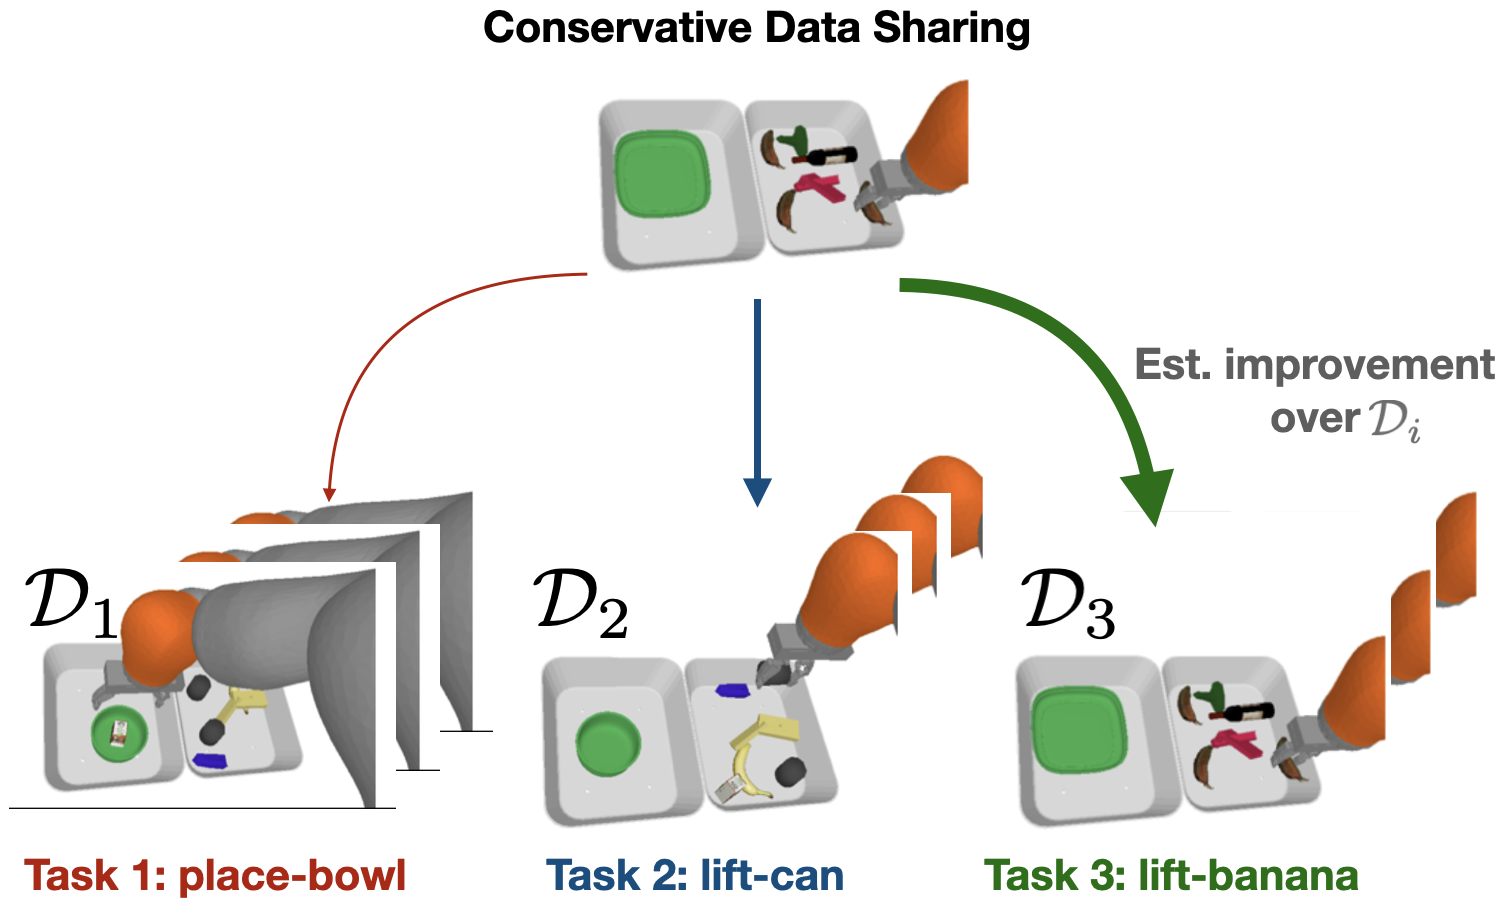
\includegraphics[width=0.45\textwidth]{chapters/cds/cds_teaser.png}
    %%SL.7.31: consider making this a wrapfigure
    \vspace{-0.2cm}
    \caption{\footnotesize A visualization of \cdsmethodname, which routes a transition to
    the offline dataset $\mathcal{D}_i$ for each task $i$ with a weight based on the estimated improvement over the behavior policy $\pi_\beta(\ba|\bs, i)$ of $\mathcal{D}_i$ after sharing the transition.}
    \label{fig:teaser}
    \vspace{-0.3cm}
\end{wrapfigure}


The main contributions of this work are an analysis of data sharing in offline multi-task RL and a new algorithm, \textit{conservative data sharing} (\cdsmethodname), for multi-task offline RL problems. \arxiv{\cdsmethodname\ relabels a transition into a given task only when it is expected to improve performance based on a conservative estimate of the Q-function.} 
After data sharing, similarly to prior offline RL methods, \cdsmethodname\ applies a standard conservative offline RL algorithm, such as CQL~\citep{kumar2020conservative}, that learns a conservative value function or BRAC~\citep{wu2019behavior}, a policy-constraint offline RL algorithm. Further, we theoretically analyze \cdsmethodname\ and characterize scenarios under which it provides safe policy improvement guarantees. Finally, we conduct extensive empirical analysis of \cdsmethodname\ on multi-task locomotion, multi-task robotic manipulation with sparse rewards, multi-task navigation, and multi-task imaged-based robotic manipulation. We compare CDS to vanilla offline multi-task RL without sharing data, to na\"{i}vely sharing data for all tasks, and to existing data relabeling schemes for multi-task RL. \cdsmethodname\ is the only method to attain good performance across all of these benchmarks, often significantly outperforming the best \textit{domain-specific} method, improving over the next best method on each domain by \textbf{17.5\%} on average.

\section{Related Work}

\textbf{Offline RL.} Offline RL~\citep{ernst2005tree, riedmiller2005neural, LangeGR12, levine2020offline} has shown promise in domains such as robotic manipulation~\citep{kalashnikov2018scalable, mandlekar2020iris, Rafailov2020LOMPO,singh2020cog,kalashnikov2021mt}, NLP~\citep{jaques2019way,jaques2020human}, recommender systems \& advertising~\citep{strehl2010learning,garcin2014offline,charles2013counterfactual,theocharous2015ad,thomas2017predictive}, and healthcare~\citep{shortreed2011informing, Wang2018SupervisedRL}. The major challenge in offline RL is distribution shift~\citep{fujimoto2018off,kumar2019stabilizing,kumar2020conservative}, where the learned policy might generate out-of-distribution actions, resulting in erroneous value backups. Prior offline RL methods address this issue by regularizing the learned policy to be ``close`` to the behavior policy~\citep{fujimoto2018off,liu2020provably,jaques2019way,wu2019behavior, zhou2020plas,kumar2019stabilizing,siegel2020keep, peng2019advantage}, through variants of importance sampling~\citep{precup2001off, sutton2016emphatic, LiuSAB19, SwaminathanJ15, nachum2019algaedice}, via uncertainty quantification on Q-values~\citep{agarwal2020optimistic, kumar2019stabilizing, wu2019behavior, levine2020offline}, by learning conservative Q-functions~\citep{kumar2020conservative,kostrikov2021offline}, and with model-based training with a penalty on out-of-distribution states~\citep{kidambi2020morel, yu2020mopo,matsushima2020deployment,argenson2020model,swazinna2020overcoming,Rafailov2020LOMPO,lee2021representation,yu2021combo}. While current benchmarks in offline RL~\citep{fu2020d4rl,gulcehre2020rl} contain datasets that involve multi-task structure, existing offline RL methods do not leverage the shared structure of multiple tasks and instead train each individual task from scratch. In this paper, we exploit the shared structure in the offline multi-task setting and train a general policy that can acquire multiple skills.

%%CF.5.17: I would consider mentioning meta-RL methods somewhere, since they also address multi-task RL and especially since there are some that aren't conflicted I think (e.g. VariBAD, meta-Q-learning). Some of them even reuse data
%%TY.5.21: I think meta-RL methods might be a bit orthogonal since they aim for generalization to new tasks. I can cite some multi-task RL works that are less conflicted.
\textbf{Multi-task RL algorithms.} Multi-task RL algorithms~\citep{wilson2007multi,parisotto2015actor,teh2017distral,espeholt2018impala,hessel2019popart,yu2020gradient, xu2020knowledge, yang2020multi, kalashnikov2021mt,sodhani2021multi}
%%CF.5.17: there are online MTRL methods that are more recent than this. For example, there's one on soft modules from USC or UCSD. You can look at papers that cite PCGrad or meta-world and/or look on google scholar for more.
%%TY.5.21: added several more papers.
focus on solving multiple tasks jointly in an efficient way. While multi-task RL methods seem to provide a promising way to build general-purpose agents~\citep{kalashnikov2021mt}, prior works have observed major challenges in multi-task RL, in particular, the optimization challenge~\citep{hessel2019popart,schaul2019ray,yu2020gradient}.
Beyond the optimization challenge, how to perform effective representation learning via weight sharing is another major challenge in multi-task RL. Prior works have considered distilling per-task policies into a single policy that solves all tasks~\citep{rusu2015policy,teh2017distral,ghosh2017divide,xu2020knowledge}, separate shared and task-specific modules with theoretical guarantees~\citep{d2019sharing}, and incorporating additional supervision~\citep{sodhani2021multi}. Finally, sharing data across tasks emerges as a challenge in multi-task RL, especially in the off-policy setting, as na\"{i}vely sharing data across all tasks turns out to hurt performance in certain scenarios~\citep{kalashnikov2021mt}. Unlike most of these prior works, we focus on the offline setting where the challenges in data sharing are most relevant. Methods that study optimization and representation learning issues are complementary and can be readily combined with our approach.
%%CF.5.17: how does your method & analysis contrast with all of these methods? need to explicitly state what is different. (ie things like - we focus on the offline setting where some of these issues are less severe & just different; we focus on data sharing & methods that look at optimization & representation are complementary, something about the analysis contributing to our understanding in a complementary way, etc)
%%CF.5.17: I also wonder if we should include a comparison that runs only one of these methods to show some evidence that they don't solve the problem.
%%TY.5.21: Added the discussion above. We can also perform the empirical analysis on HIPI to see if it solves the problem.
% We will next survey methods in data sharing in multi-task off-policy RL.

%%CF.5.17: Other papers that do some form of data sharing:
% the REPAINT paper - includes a less naive data sharing approach
% model-based RL methods (e.g. visual foresight, some experiments in Danijar's papers, MBOLD) - these share everything
% Dave Held paper on goal-conditioned RL from images - not sure how they share
% probably other GCRL papers? eg Yevgen's actionable models, distributional planning networks, but probably others that aren't conflicted
%%TY.5.21: The REPAINT paper and model-based RL methods do not seem to study the multi-task problem, which might be less relevant? I added references to more GCRL papers.
%%CF.8.1: The model-based RL papers that I mention above *do* include some multi-task experiments (and share data across tasks, and often don't recompute rewards because often only the model is what is sharing cross-task data.) Also, both visual foresight and MBOLD operate in the fully offline setting.
\textbf{Data sharing in multi-task RL.} Prior works~\citep{andrychowicz2017hindsight,kaelbling1993learning,pong2018temporal,schaul2015universal,eysenbach2020rewriting,li2020generalized,kalashnikov2021mt,chebotar2021actionable} have found it effective to reuse data across tasks by recomputing the rewards of data collected for one task and using such relabeled data for other tasks, which effectively augments the amount of data available for learning each task and boosts performance. These methods perform relabeling either uniformly~\citep{kalashnikov2021mt} or based on metrics such as estimated Q-values~\citep{eysenbach2020rewriting,li2020generalized}, domain knowledge~\citep{kalashnikov2021mt}, the distance to states or images in goal-conditioned settings~\citep{andrychowicz2017hindsight,pong2018temporal,nair2018visual,liu2019competitive,sun2019policy,lin2019reinforcement,huang2019mapping,lynch2020grounding,yang2021bias,chebotar2021actionable}, \arxiv{and metric learning for robust inference in the offline meta-RL setting~\citep{li2019multi}. All of these methods either require online data collection and do not consider data sharing in a fully offline setting, or only consider offline goal-conditioned or meta-RL problems~\citep{chebotar2021actionable,li2019multi}.} \arxiv{While these prior works empirically find that data sharing helps, we believe that our analysis in Section~\ref{sec:analysis} provides the first analytical understanding of why and when data sharing can help in multi-task offline RL and why it hurts in some cases.} 
\arxiv{Specifically, our analysis reveals the effect of distributional shift introduced during data sharing, which is not taken into account by these prior works. Our proposed approach, CDS, tackles the challenge of distributional shift in data sharing by intelligently sharing data across tasks and improves multi-task performance by effectively trading off between the benefits of data sharing and the harms of excessive distributional shift.}
%%SL.8.1: I think this paragraph kind of buries the main point: it makes it sound like we are just (rather naively) extending the ideas from these past papers to the offline multi-task setting, which really undersells the contribution. It's not like we're just doing what they already did but extending beyond goals, we are actually addressing a challenge that these methods did not address (and indeed that they suffer from).
%%TY.8.1: I revised the above paragraph to say that our method addresses the challenge that prior works didn't address.
%%SL.5.15: I think it's important to expand the discussion of prior multi-task RL methods and better cover other methods that aim to understand why multi-task RL is hard, empirically observe that it's hard, and offer various solutions. Right now the above citations seem to focus more or less exclusively on "applications" of multi-task RL, whereas we need to survey prior work on analysis and solutions (maybe in a separate paragraph). This includes things like ray interference, pcgrad, and other papers you can find that cite those or are cited by them
%%TY.5.16: I added a paragraph discussing challenges in multi-task RL and then use the above paragraph to survey relabeling methods in the off-policy setting.


\vspace{-5pt}
\section{Preliminaries and Problem Statement}
\vspace{-5pt}
\label{sec:prelims}
% In this section, we introduce notation, present our problem formulation, and review the base offline RL methods that our algorithm utilizes.

\textbf{Multi-task offline RL.} The goal in multi-task RL is to find a policy that maximizes expected return in a multi-task Markov decision process (MDP), defined as   $\mdp =(\states, \actions, P, \gamma, \{R_i, i \}_{i=1}^N)$, with state space $\states$, action space $\actions$, dynamics $P(\bs' | \bs, \mathbf{a})$, a discount factor $\gamma \in [0, 1)$, and a finite set of task indices $1, \cdots, N$
with corresponding reward functions $R_1, \cdots, R_N$. Each task $i$ presents a different reward function $R_i$, but we assume that the dynamics $P$ are shared across tasks. While this setting is not fully general, there are a wide variety of practical problem settings for which only the reward changes including various goal navigation tasks~\cite{fu2020d4rl}, distinct object manipulation objectives~\cite{xie2018few}, and different user preferences~\cite{christiano2017deep}.
In this work, we focus on learning a policy $\pi(\mathbf{a}|\bs, i)$, which in practice could be modelled as independent policies $\{\pi_1(\mathbf{a}|\bs), \cdots, \pi_N(\mathbf{a}|\bs)\}$ that do not share any parameters, or as a single task-conditioned policy, $\pi(\mathbf{a}|\bs, i)$ with parameter sharing. Our goal in this paper is to analyze and devise methods for data sharing and the choice of parameter sharing is orthogonal, and can be made independently.
We formulate the policy optimization problem as finding a policy that maximizes expected return over all the tasks: $\pi^*(\mathbf{a}|\bs, \cdot) := \arg \max_{\pi} \mathbb{E}_{i \sim [N]} \mathbb{E}_{\pi(\cdot|\cdot, i)}[\sum_{t} \gamma^t R_i(\bs_t, \mathbf{a}_t)]$.
The Q-function, $Q^\pi(\bs, \mathbf{a}, i)$, of a policy $\pi(\cdot|\cdot, i)$ is the long-term discounted reward obtained in task $i$ by executing action $\mathbf{a}$ at state $\bs$ and following policy $\pi$ thereafter.
%%CF.5.22: the above paragraph seems to be a lot more than just notation and definitions, especially the part about the reward being the same across tasks (since that is part of our problem definition). How about you have the multi-task offline RL paragraph header for this paragraph? (and then no header for the next paragraph)
%%CF.5.22: Need to make it clear that we assume that we know the form of the reward function r_i, a common assumption in goal-conditioned RL~\cite{}, and which often holds in robotics applications through the use of learned classifiers~\cite{annie_flo,qtopt} and discriminators~\cite{vice,chen_dvd}.

%%SL.5.23: A subtlety in the problem formulation: a "task conditioned policy" is really just an architectural choice. Basically, we have a different policy for each task, but these policies may share parameters. It might be good to explain this detail though, because the point of our paper is how to share data, *not* how to share model weights. So in principle all this stuff would apply just as well if we had totally separate policies per task.

Standard offline RL is concerned with learning policies $\pi(\mathbf{a}|\bs)$ using only a given static dataset of transitions $\mathcal{D} =  \{(\bs_j, \mathbf{a}_j, \bs'_j, r_j)\}_{j=1}^N$, collected by a behavior policy $\pi_\beta(\mathbf{a}|\bs)$, without any additional environment interaction. In the multi-task offline RL setting, the dataset $\mathcal{D}$ is partitioned into per-task subsets, $\mathcal{D} = \cup_{i=1}^N \mathcal{D}_i$,
where $\mathcal{D}_i$ consists of experience from task $i$. While algorithms can choose to train the policy for task $i$ (i.e., $\pi(\cdot|\cdot, i)$) only on $\mathcal{D}_{i}$, in this paper, we are interested in data-sharing schemes that correspond to relabeling data from a different task, $j \neq i$ with the reward function $r_i$, and learn $\pi(\cdot|\cdot, i)$ on the combined data. To be able to do so, we assume access to the functional form of the reward $r_i$, a common assumption in goal-conditioned RL~\cite{andrychowicz2017hindsight,eysenbach2020rewriting}, and which often holds in robotics applications through the use of learned classifiers~\cite{xie2018few,kalashnikov2018scalable}, and discriminators~\cite{fu2018variational,chen2021learning}.

We assume that relabeling data $\mathcal{D}_j$ from task $j$ to task $i$ generates a dataset $\mathcal{D}_{j \rightarrow i}$, which is then additionally used to train on task $i$. Thus, the effective dataset for task $i$ after relabeling is given by $\mathcal{D}^\mathrm{eff}_i := \mathcal{D}_i \cup \left( \cup_{j \neq i} \mathcal{D}_{j \rightarrow i} \right)$. This notation simply formalizes data sharing and relabeling strategies explored in prior work~\citep{eysenbach2020rewriting,kalashnikov2021mt}. Our aim in this paper will be to improve on this na\"{i}ve strategy, which we will show leads to significantly better results. 

\textbf{Offline RL algorithms.} A central challenge in offline RL is distributional shift: differences between the learned policy and the behavior policy can lead to erroneous target values, where the Q-function is queried at actions $\mathbf{a} \sim \pi(\mathbf{a}|\bs)$ that are far from the actions it is trained on, leading to massive overestimation~\citep{levine2020offline,kumar2019stabilizing}.
A number of offline RL algorithms use some kind of regularization on either the policy~\citep{kumar2019stabilizing,fujimoto2018off,wu2019behavior,jaques2019way,siegel2020keep,peng2019advantage} or on the learned Q-function~\citep{kumar2020conservative,kostrikov2021offline} to ensure that the learned policy does not deviate too far from the behavior policy. For our analysis in this work, we will abstract these algorithms into a generic constrained policy optimization problem~\citep{kumar2020conservative}:
\begin{equation}
\label{eqn:generic_offline_rl}
    \pi^*(\mathbf{a}|\bs) := \arg \max_{\pi}~~ J_{\mathcal{D}}(\pi) - \alpha D(\pi, \pi_\beta).
    %%SL.5.23: maybe label it as "offline RL with a policy constraint" or something?
\end{equation}
$J_{\mathcal{D}}(\pi)$ denotes the average return of policy $\pi$ in the empirical MDP induced by the transitions in the dataset, and $D(\pi, \pi_\beta)$ denotes a divergence measure (e.g., KL-divergence~\citep{jaques2019way,wu2019behavior}, MMD distance~\citep{kumar2019stabilizing} or $D_{\text{CQL}}$~\citep{kumar2020conservative}) between the learned policy $\pi$ and the behavior policy $\pi_\beta$. 
% With the goal of maximizing the actual return of the policy $J(\pi) = \mathbb{E}_{\pi}[\sum_t \gamma^t r(\bs_t, \mathbf{a}_t)]$,
%%SL.5.23: This sentence is ordered backwards, the first clause should come at the end...
% but with access only to a finite dataset, these algorithms can generally be viewed as solving some instantiation of the following policy-optimization problem~\citep{kumar2020conservative}, which provides certain policy improvement guarantees~\citep{laroche2019safe,petrik2016safe,kumar2020conservative}:
% \begin{equation}
% \label{eqn:generic_offline_rl}
%     \pi^*(\mathbf{a}|\bs) := \arg \max_{\pi}~~ J_{\mathcal{D}}(\pi) - \alpha D(\pi, \pi_\beta)~~~~~~~~~~~~~ \text{(Offline RL)}.
%     %%SL.5.23: maybe label it as "offline RL with a policy constraint" or something?
% \end{equation}
% $J_{\mathcal{D}}(\pi)$ denotes the average return of policy $\pi$ in the empirical MDP induced by the transitions in the dataset, and $D(\pi, \pi_\beta)$ denotes a divergence measure (e.g., KL-divergence~\citep{jaques2019way}, MMD distance~\citep{kumar2019stabilizing}) between the learned policy $\pi$ and the behavior policy $\pi_\beta$. 
In the multi-task offline RL setting with data-sharing, the generic optimization problem in Equation~\ref{eqn:generic_offline_rl} for a task $i$ utilizes the effective dataset $\mathcal{D}^\mathrm{eff}_i$. In addition, we define $\pi_\beta^\mathrm{eff}(\mathbf{a}|\bs, i)$ as the effective behavior policy for task $i$ and it is given by: $\pi_\beta^\mathrm{eff}(\mathbf{a}|\bs, i) := |\mathcal{D}^\mathrm{eff}_i(\bs, \mathbf{a})| / |\mathcal{D}^\mathrm{eff}_i(\bs)|$. Hence, the counterpart of Equation~\ref{eqn:generic_offline_rl} in the multi-task offline RL setting with data sharing is given by:
\begin{equation}
\label{eqn:generic_multitask_offline_rl}
     \forall i \in [N], ~~\pi^*(\mathbf{a}|\bs, i) := \arg \max_{\pi}~~ J_{\mathcal{D}^\mathrm{eff}_i}(\pi) - \alpha D(\pi, \pi^\mathrm{eff}_\beta).
     %%CF.5.22: are J_\data(\pi, \task_i) and D(\pi, \pi_\beta; \mathcal{T}_i) ever defined? and should it be J_\mathcal{D} or J_\mathcal{D}(\task) or something else?
\end{equation}
We will utilize this generic optimization problem to motivate our method in Section~\ref{sec:method}.

% Given an MDP $\mdp =(\states, \actions, R, P, \gamma)$ \citep{puterman1994markov}, with state space $\states$, action space $\actions$, a reward function $R(\bs, \mathbf{a})$, dynamics $P(\bs' | \bs, \mathbf{a})$ and a discount factor $\gamma \in [0, 1)$, the goal of  The Q-function $Q^\pi(\bs, \mathbf{a})$ for a policy $\pi(\mathbf{a}|\bs)$ is the expected long-term discounted reward obtained by executing action $\mathbf{a}$ at state $\bs$ and following $\pi(\mathbf{a}|\bs)$ thereafter, 
% $Q^\pi(\bs, \mathbf{a}) := \E\left[ \sum\nolimits_{t=0}^\infty \gamma^t R(\bs_t, \mathbf{a}_t) \right]$.

%%CF.5.18: I think it's pretty important to define the problem statement here. We do make the assumption that only the reward varies across tasks, and that we have access to the reward function. These assumptions aren't entirely standard in MTRL, so it's important to be upfront about them. (It could also make sense to include a mention of it in the intro, so that we are even more upfront about it)

% \begin{wrapfigure}{r}{7cm}
%   \vspace{-0.3cm}
%   \centering
%   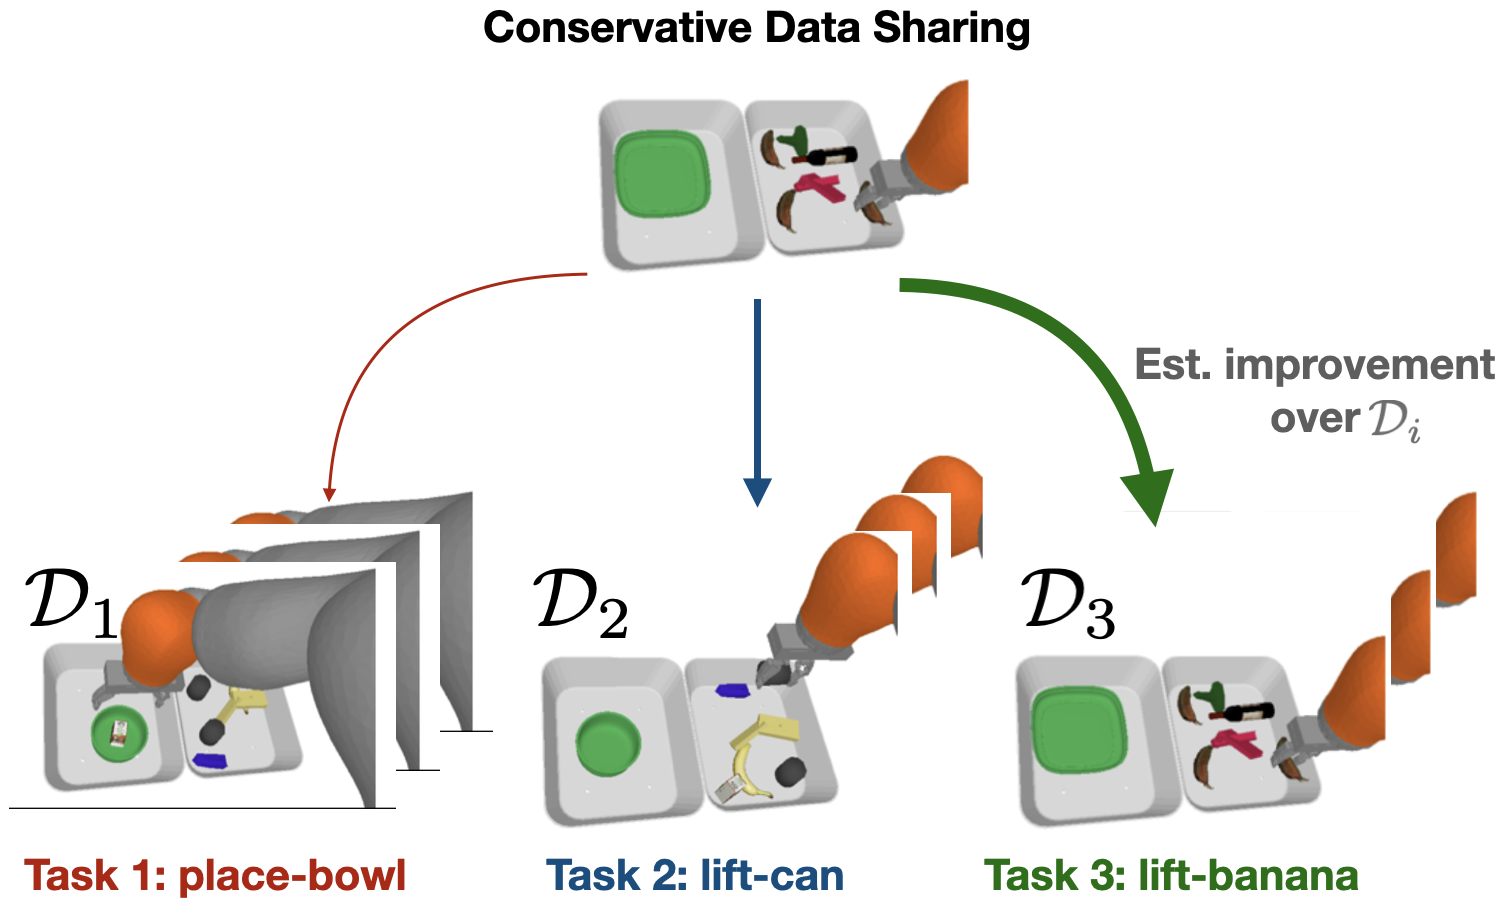
\includegraphics[width=0.45\textwidth]{chapters/cds/cds_teaser.png}
%   %%SL.7.31: consider making this a wrapfigure
%   \vspace{-0.2cm}
%   \caption{\footnotesize A visualization of \cdsmethodname, which routes a transition to
%   the offline dataset $\mathcal{D}_i$ for each task $i$ with a weight based on the estimated improvement over the behavior policy $\pi_\beta(\ba|\bs, i)$ of $\mathcal{D}_i$ after sharing the transition.}
%   \label{fig:teaser}
%   \vspace{-0.3cm}
% \end{wrapfigure}


\subsection{When Does Data Sharing Actually Help in Offline Multi-Task RL?}
\label{sec:analysis}
\vspace{-0.1cm}

Our goal is to leverage experience from all tasks to learn a policy for a particular task of interest. Perhaps the simplest approach to leveraging experience across tasks is to train the task policy on not just the data coming from that task, but also relabeled data from all other tasks~\citep{caruana1997multitask}. Is this na\"ive data sharing strategy sufficient for learning effective behaviors from multi-task offline data? In this section, we aim to answer this question via empirical analysis on a relatively simple domain, which will reveal interesting aspects of data sharing. We first describe the experimental setup and then discuss the results and possible explanations for the observed behavior. Using insights obtained from this analysis, we will then derive a simple and effective data sharing strategy in Section~\ref{sec:method}.

\textbf{Experimental analysis setup.} To assess the efficacy of data sharing, we experimentally analyze various multi-task RL scenarios created with the walker2d environment in Gym~\citep{brockman2016openai}. We construct different test scenarios on this environment that mimic practical situations, including settings where different amounts of  data of varied quality are available for different tasks~\citep{kalashnikov2021mt,xie2019improvisation,singh2020parrot}. In all these scenarios, the agent attempts three tasks: \texttt{run forward}, \texttt{run backward}, and \texttt{jump}, which we visualize in Figure~\ref{fig:env}. Following the problem statement in Section~\ref{sec:prelims}, these tasks share the same state-action space and transition dynamics, differing only in the reward function that the agent is trying to optimize. 
Different scenarios are generated with varying size offline datasets, each collected with policies that have different degrees of suboptimality. This might include, for each task, a single policy with mediocre or expert performance, or a mixture of policies given by the initial part of the replay buffer trained with online SAC~\citep{haarnoja2018soft}. We refer to these three types of offline datasets as medium, expert and medium-replay, respectively, following \citet{fu2020d4rl}.

We train a single-task policy $\pi_\mathrm{CQL}(\mathbf{a}|\bs, i)$ with CQL~\citep{kumar2020conservative} as the base offline RL method, along with two forms of data-sharing, as shown in Table~\ref{tab:analysis}: no sharing of data across tasks (\textbf{No Sharing}) and complete sharing of data with relabeling across all tasks (\textbf{Sharing All}). In addition, we also measure the divergence term in Equation~\ref{eqn:generic_multitask_offline_rl}, $D(\pi(\cdot|\cdot, i), \pi^\mathrm{eff}_\beta(\cdot|\cdot, i))$, for $\pi = \pi_\mathrm{CQL}(\mathbf{a}|\bs, i)$, averaged across tasks by using the
Kullback-Liebler divergence. This value quantifies the average divergence between the single-task optimal policy and the relabeled behavior policy averaged across tasks.  

\begin{table*}[t]
\centering
\scriptsize
\def\arraystretch{0.9}
\setlength{\tabcolsep}{0.42em}
\resizebox{0.95\textwidth}{!}{\begin{tabular}{cc|cc|cc}
  \toprule
 \multicolumn{1}{c}{\multirow{1.5}[2]{*}{Dataset types / Tasks}} & \multicolumn{1}{c}{\multirow{1.5}[2]{*}{Dataset Size}}\vline &
 \multicolumn{2}{c}{Avg Return}\vline & \multicolumn{2}{c}{$D_\text{KL}(\pi, \pi_\beta)$}\\
 & \multicolumn{1}{c}{}\vline & \multicolumn{1}{c}{\textbf{No Sharing}}  & \multicolumn{1}{c}{\textbf{Sharing All}}\vline  & \multicolumn{1}{c}{\textbf{No Sharing}}  & \multicolumn{1}{c}{\textbf{Sharing All}} \\
\midrule
  medium-replay / \texttt{run forward} & 109900 & \textbf{998.9} & 966.2 & \textbf{3.70} & 10.39\\
  medium-replay / \texttt{run backward} & 109980 & \textbf{1298.6} & 1147.5 & \textbf{4.55} & 12.70\\
  medium-replay / \texttt{jump} & 109511 & \textbf{1603.1} & 1224.7 & \textbf{3.57} & 15.89\\
  \rowcolor{Gray}
  \textbf{average task performance} & N/A & \textbf{1300.2} & 1112.8 & \textbf{3.94}  & 12.99\\
  \midrule
  medium / \texttt{run forward} & 27646 & 297.4  & \textbf{848.7} &\textbf{6.53} & 11.78\\
  medium / \texttt{run backward} & 31298 & 207.5 & \textbf{600.4}& \textbf{4.44} & 10.13\\
  medium / \texttt{jump} & 100000 & 351.1 & \textbf{776.1}& \textbf{5.57} & 21.27\\
%   \hline
\rowcolor{Gray}
  \textbf{average task performance} & N/A & 285.3 & \textbf{747.7} & \textbf{5.51} & 14.39 \\
  \midrule
  medium-replay / \texttt{run forward} & 109900 & 590.1 & \textbf{701.4}& \textbf{1.49} & 7.76\\
  medium / \texttt{run backward} & 31298 & 614.7 & \textbf{756.7}& \textbf{1.91} & 12.2\\
  \rowcolor{yellow}
  expert / \texttt{jump} & 5000 & \textbf{1575.2} & 885.1 & \textbf{3.12} & 27.5\\
%   \hline
\rowcolor{Gray}
  \textbf{average task performance} & N/A & \textbf{926.6} & 781 & \textbf{2.17}  & 15.82 \\
    \bottomrule
\end{tabular}}
    \vspace{-0.1cm}
         \caption{\footnotesize We analyze how sharing data across all tasks (\textbf{Sharing All}) compares to \textbf{No Sharing} in the multi-task walker2d environment with three tasks: run forward, run backward, and jump. We provide three scenarios with different styles of per-task offline datasets in the leftmost column. The second column shows the number of transitions in each dataset. We report the per-task average return, the KL divergence between the single-task optimal policy $\pi$ and the behavior policy $\behavior$ after the data sharing scheme, as well as averages across tasks. \textbf{Sharing All} generally helps training while increasing the KL divergence. However, on the row highlighted in yellow, \textbf{Sharing All} yields a particularly large KL divergence between the single-task $\pi$ and $\behavior$ and degrades the performance, suggesting sharing data for all tasks is brittle.
     \label{tab:analysis}
     \vspace{-0.2cm}
     }
\end{table*}

\textbf{Analysis of results in Table~\ref{tab:analysis}.} To begin, note that even na\"ively sharing data is  better than not sharing any data at all on \textbf{5/9} tasks considered
(compare the performance across \textbf{No Sharing} and \textbf{Sharing All} in Table~\ref{tab:analysis}). However, a closer look at Table~\ref{tab:analysis} suggests that data-sharing can significantly degrade performance on certain tasks, especially in scenarios where the amount of data available for the original task is limited, and where the distribution of this data is narrow.
For example, when using expert data for jumping in conjunction with more than 25 times as much lower-quality (mediocre \& random) data for running forward and backward, we find that the agent performs poorly on the jumping task despite access to near-optimal jumping data.

~

\niparagraph{\emph{Why does na\"ive data sharing degrade performance on certain tasks despite near-optimal behavior for these tasks in the original task dataset?}} We argue that the primary reason that na\"{i}ve data sharing can actually hurt performance in such cases is because it exacerbates the distributional shift issues that afflict offline RL. Many offline RL methods combat distribution shift by implicitly or explicitly constraining the learned policy to stay close to the training data. Then, when the training data is changed by adding relabeled data from another task, the constraint causes the learned policy to change as well. When the added data is of low quality for that task, it will correspondingly lead to a lower quality learned policy for that task, unless the constraint is somehow modified. This effect is evident from the higher divergence values between the learned policy without any data-sharing and the effective behavior policy for that task \emph{after} relabeling (e.g., expert+\texttt{jump}) in Table~\ref{tab:analysis}. Although these results are only for CQL, we expect that any offline RL method would, insofar as it combats distributional shift by staying close to the data, would exhibit a similar problem. 


\niparagraph{\textbf{To mathematically quantify}} the effects of data-sharing in multi-task offline RL, we appeal to safe policy improvement bounds~\citep{laroche2019safe,kumar2020conservative,yu2021combo} and discuss cases where data-sharing between tasks $i$ and $j$ can degrade the amount of worst-case guaranteed improvement over the behavior policy. Prior work~\citep{kumar2020conservative} has shown that the generic offline RL algorithm in Equation~\ref{eqn:generic_offline_rl} enjoys the following guarantees of policy improvement on the actual MDP, beyond the behavior policy: 
\begin{align}
\label{eqn:spi}
    J(\pi^*) &\geq J(\pi_\beta) - \mathcal{O}(1/ (1 - \gamma)^2) \mathbb{E}_{\bs, \mathbf{a} \sim d^{\pi}} \left[\sqrt{\frac{D(\pi(\cdot|\bs), \pi_\beta(\cdot|\bs))}{|\mathcal{D}(\bs)|}}\right] + \alpha/(1 - \gamma) D(\pi, \pi_\beta).
\end{align}
We will use Equation~\ref{eqn:spi} to understand the scenarios where data sharing can hurt. When data sharing modifies $\mathcal{D} = \mathcal{D}_i$ to $\mathcal{D} = \mathcal{D}^\mathrm{eff}_i$, which includes $\mathcal{D}_i$ as a subset, it effectively aims at reducing the magnitude of the second term (i.e., sampling error) by increasing the denominator. This can be highly effective if the state distribution of the learned policy $\pi^*$ and the dataset $\mathcal{D}$ overlap. However, an increase in the divergence $D(\pi(\cdot|\bs), \pi^\beta(\cdot|\bs))$ as a consequence of relabeling implies a potential increase in the sampling error, unless the increased value of $|\mathcal{D}^\mathrm{eff}(\bs)|$ compensates for this. Additionally, the bound also depends on the quality of the behavior data added after relabeling: if the resulting behavior policy $\pi^\mathrm{eff}_\beta$ is more suboptimal compared to $\pi_\beta$, i.e., $J(\pi^\mathrm{eff}_\beta) < J(\pi_\beta)$, then the guaranteed amount of improvement also reduces.

% \begin{proposition}[Na\"ive data-sharing can hurt policy performance.] Assume that the the multi-task MDP consists of discrete states $\mathcal{S}$ and actions $\mathcal{A}$. Consider the scenario where data from task $\mathcal{T}_j$, $\mathcal{D}(\mathcal{T}_j)$, is relabelled to task $\mathcal{T}_i$ and let $\mathcal{D}_\mathrm{eff}(\mathcal{T}_i) = \mathcal{D}(\mathcal{T}_j \rightarrow \mathcal{T}_i) \cup \mathcal{D}(\mathcal{T}_i)$. For any dataset, let $|\mathcal{D}(\bs)|$ be the frequency of a state $\bs$ in $\mathcal{D}$, $\pi^*(\mathbf{a}|\bs, \mathcal{T}_i)$ denote the optimal solution to Equation~\ref{eqn:generic_multitask_offline_rl} without any data sharing and let $\pi^*_\mathrm{eff}(\mathbf{a}|\bs)$ be the optimal solution of Equation~\ref{eqn:generic_multitask_offline_rl} with data sharing. Let $\pi^\mathrm{eff}_\beta(\mathbf{a}|\bs, \mathcal{T}_i)$ denote the effective behavior policy for $\mathcal{D}_\mathrm{eff}(\mathcal{T}_i)$. Then, sharing data from task $\mathcal{T}_j$ to task $\mathcal{T}_i$ may not improve the resulting policy performance on task $\mathcal{T}_i$, i.e., $J(\pi^*, \mathcal{T}_i) \geq J(\pi^*_\mathrm{eff}, \mathcal{T}_i) + \zeta$, in the worst-case where:
% \begin{equation*}
%     \zeta \geq  C \mathbb{E}_{\bs, \mathbf{a} \sim d^{\pi^*}} \left[ \sqrt{\frac{D(\pi(\cdot|\bs), \pi^\mathrm{eff}_\beta(\cdot|\bs))}{{|\mathcal{D}_\mathrm{eff}(\mathcal{T}_i)(\bs)|}}} \right] - C \mathbb{E}_{\bs, \mathbf{a} \sim d^{\pi^*}} \left[ \sqrt{\frac{D(\pi(\cdot|\bs), \pi_\beta(\cdot|\bs))}{{|\mathcal{D}(\mathcal{T}_i)(\bs)|}}} \right] + J_{\mathcal{T}_i}(\pi_\beta) - J_{\mathcal{T}_i}(\pi_\beta^\mathrm{eff}) 
% \end{equation*}
% where $C$ is a universal constant depending on the MDP, $d^{\pi^*}$ denotes the state-action marginal of policy $\pi^*$ on the MDP and $\varepsilon > 0$.
% \label{prop:data_sharing}
% \end{proposition}
% While the inequality in Proposition~\ref{prop:data_sharing} is only a bound on performance, it still reveals some tradeoffs associated with data sharing: when data sharing induces distributional shift, such that the value of $D(\pi, \pi^\mathrm{eff}_\beta)$ increases compared to $D(\pi, \pi_\beta)$, without increasing visitation frequencies of states under the learned single-task policy, such that $|\mathcal{D}_\mathrm{eff}(\mathcal{T}_i)(\bs)|$ does not increase enough
% beyond $|\mathcal{D}(\mathcal{T}_i)(\bs)|$ to compensate for the increase in $D(\pi, \pi^\mathrm{eff}_\beta)$, poor performance might be obtained.
% %%SL.5.23: what about the proposition indicates that poor performance might be obtained? can we make this part of the statement more precise?
% The performance decrease is exacerbated when the data being shared is of low quality, i.e., $J(\pi_\beta^\mathrm{eff}) \leq J(\pi_\beta)$. 
% %%AK: maybe we should also have a figure illustrating the spectrum of data-sharing: there is an optimistic end, share everything, a conservative end, share nothing and the more conservative side of the spectrum where our method lies? This is kinda like what I had drawn earlier on the jamboard notes when we discussed a few months back.

% Two considerations: (1) task alignment (2) different dataset types, which can hurt optimziation. Summarioze the main "rules", phenomenon by this this happens. Consequences -- conservative or you become optimistic, etc
% To conclude, we observe that while na\"ive data sharing can generally help improve performance in multi-task offline RL, but that the behavior policy coupled with the amount of data observed can have a significant impact on the performance of na\"ive data sharing. This may prevent existing algorithms from leveraging large pre-existing datasets of potentially useful, but not directly-relevant behaviors to improve performance, thereby hindering generalization. In the next section, we present our method, \cdsmethodname,  that addresses this issue and is derived via a principled optimization problem that aims to maximize per-task performance.

\textbf{To conclude,} our analysis reveals that while data sharing is often helpful in multi-task offline RL, it can lead to substantially poor performance on certain tasks as a result of exacerbated distributional shift between the optimal policy and the effective behavior policy induced after sharing data. 
% Thus, in order to obtain effective policies for all tasks in this setting, we propose to share data \emph{conservatively},
% with precaution taken to not exacerbate distributional shift via relabeling. This forms the basis of our data-sharing scheme, \cdsmethodname, which we will discuss next.

% \vspace{-5pt}
% \section{Regimes of Data Sharing in Multi-Task Offline RL}
% \label{sec:different_regimes}
% The analysis in Section~\ref{sec:analysis} shows that na\"ive data sharing may be highly sub-optimal in some cases, and although it often does improve over no data sharing at all in practice, it can also lead to exceedingly poor performance. On the other hand, no data sharing can also lead to poor performance since it is overly conservative, and does not share any experience at all. In this section, we aim to understand the spectrum in between no data sharing and complete data sharing, aiming to understand the kinds of data sharing schemes that provide a balanced tradeoff between no data sharing and full data sharing. We will then use the insights gathered from this section to derive a complete method in Section~\ref{sec:method}.

% Since full data sharing exacerbates distributional shift, a simple data sharing strategy could be to share data only when distributional shift is reduced. That is, more formally, for any given transition $(\bs, \mathbf{a}, r, \bs')$, this scheme would compare $D(\pi, \pi_\beta)(\bs)$ and $D(\pi, \pi^{\text{eff}}_\beta)(\bs)$ and utilize the transition for training only when $D(\pi, \pi_\beta)(\bs) \geq D(\pi, \pi_\beta^\text{eff})(\bs)$. We refer to this scheme as X. 

% While X provably alleviates the concerns of increasing distribution shift as a result of data sharing, it is overly conservative in practice. A distinct, more optimistic scheme for data sharing is to share a use a transition $(\bs, \mathbf{a}, r, \bs')$ for training only if the resulting data improves upon the learned policy performance.   

\vspace{-5pt}
\subsection{\cdsmethodname: Reducing Distributional Shift in Multi-Task Data Sharing}
\label{sec:method}
\vspace{-5pt}
The analysis in Section~\ref{sec:analysis} shows that na\"ive data sharing may be highly sub-optimal in some cases, and although it often does improve over no data sharing at all in practice, it can also lead to exceedingly poor performance. Can we devise a conservative approach that shares data intelligently to not exacerbate distributional shift as a result of relabeling?
%%CF.8.1: This question above is super long, and starts to get incomprehensible towards the end. Can you shorten or split it up? And, what's the difference between the benefits of sharing data and the benefits of sharing data of high quality?? I think that my suggested edit should fix this.
%%AK: addressed, just kept the first part of this since the story of quality and sampling error comes in after 5.1

\subsubsection{A First Attempt at Designing a Data Sharing Strategy}
A straightforward data sharing strategy is to utilize a transition for training only if it reduces the distributional shift.
%%SL.8.1: The above sentence comes across as a bit obtuse -- of course doing X only if it reduces distributional shift will, by definition, not increase distributional shift -- can you rephrase?
%%CF.8.1: +1. Maybe "A starightforward data sharing strategy is to utilize a transition for training only if it reduces the distribution shift."
%%AK: done
Formally, this means that for a given transition $(\bs, \mathbf{a}, r_j(\bs, \mathbf{a}), \bs') \in \mathcal{D}_j$ sampled from the dataset $\mathcal{D}_j$, such a scheme would prescribe using it for training task $i$ (i.e., $(\bs, \mathbf{a}, r_i(\bs, \mathbf{a}), \bs') \in \mathcal{D}^\mathrm{eff}_i$) only if: 
%%CF.8.1: can you simplify the structure of the above sentence? it is a lot to take in and will probably require the reader to read it twice in its current form.
%%AK: slightly reogranized. Is it still too hard to read?
\begin{tcolorbox}[colback=blue!6!white,colframe=black,boxsep=0pt,top=-3pt,bottom=2pt]
\begin{equation}
\label{eqn:pessimistically_conservative}
    \text{\textbf{CDS (basic)}:}~~~~~~~\Delta^\pi(\bs, \mathbf{a}) := D(\pi(\cdot|\cdot, i), \pi_\beta(\cdot|\cdot, i))(\bs) - D(\pi(\cdot|\cdot, i), \pi_\beta^{\text{eff}}(\cdot|\cdot, i))(\bs) \geq 0. 
\end{equation}
\end{tcolorbox}
%%AK: the above equation is not technically correct, since there is no a on the right side of \Delta^\pi(s, a), need to fix this.
The scheme presented in Equation~\ref{eqn:pessimistically_conservative} would guarantee that distributional shift (i.e., second term in Equation~\ref{eqn:generic_multitask_offline_rl}) is reduced.
%%CF.8.1: i.e. that distribution shift is reduced.
%%AK: done
Moreover, since sharing data can only increase the size of the dataset and not reduce it, this scheme is guaranteed to not increase the sampling error term in Equation~\ref{eqn:spi}. We refer to this scheme as the basic variant of conservative data sharing (\textbf{CDS (basic)}).
%%CF.8.1: hmm, I wouldn't recommend forward referencing equations like this.
%%AK: this was an error in the equatino refercing, this question appears before.

While this scheme can prevent the negative effects of increased distributional shift, this scheme is quite pessimistic. Even in our experiments, we find that this variant of CDS does not improve performance by a large margin.
%%TY.8.2: did our experiments show this? Maybe we should rephrase to "we find that this variant of CDS performs underwhelmingly, achieving worse results compared to the naively data sharing and no data sharing approaches".
%%AK: done
Additionally, as observed in Table~\ref{tab:analysis} (medium-medium-medium data composition) and discussed in Section~\ref{sec:analysis}, data sharing can often be useful despite an increased distributional shift (note the higher values of $D_\mathrm{KL}(\pi, \pi_\beta)$ in Table~\ref{tab:analysis}) likely because it reduces sampling error and potentially utilizes data of higher quality for training. \textbf{CDS (basic)} described above does not take into account these factors. Formally, the effect of the first term in Equation~\ref{eqn:generic_multitask_offline_rl}, $J_{\mathcal{D}^\text{eff}}(\pi)$ (the policy return in the empirical MDP generated by the dataset) and a larger increase in $|\mathcal{D}^\mathrm{eff}(\bs)|$ at the cost of somewhat increased value of $D(\pi(\cdot|\bs), \pi_\beta(\cdot|\bs)$ are not taken into account. Thus we ask: can we instead design a more complete version of CDS that effectively balances the tradeoff by incorporating all the discussed factors (distributional shift, sampling error, data quality)?  
% This term is guaranteed to increase with the scheme in Equation~\ref{eqn:pessimistically_conservative} in practice, since this scheme only utilizes \emph{additional} data corresponding to other tasks for training which would not reduce the performance of the policy compared to no sharing. Combined with the reduced value of the second term, this implies that this scheme increases the objective in Equation~\ref{eqn:generic_multitask_offline_rl}. 

%%SL.8.1: In the interest of space, I think this paragraph can largely be cut, since the end of the previous paragraph already motivates the need for a less conservative method. You could cut this and replace it with a sentence or two at the beginning of the next section.
%%CF.8.1: +1
% \textbf{Is p-CDS sufficient for effective multi-task offline RL?} While p-CDS guarantees that the shared data will not exacerbate distributional shift, which is quite useful in cases such as the walker2d expert scenario analyzed in Section~\ref{sec:analysis}, this scheme can be overly pessimistic. As we also find in our experiments in Section~\ref{sec:exp}, p-CDS often chooses to not share any data in scenarios where it is impossible to meet the strong requirement of reduced distributional shift. On the other side, in a number of scenarios, data sharing improves performance because more training data stabilizes training and reduces sampling error and improves the quality of the data in the dataset, albeit at the cost of slightly increased distributional shift. This raises the question: Can we devise a conservative data sharing scheme that instead \emph{optimistically} shares data, by effectively balancing the improvement due to reduced sampling error and increased data quality, and a deterioration due to increased distributional shift? Such an optimistic scheme would not only reduce the second term in Equation~\ref{eqn:generic_multitask_offline_rl}, but would also share data if the gain in the first term $J_{\mathcal{D}^\text{eff}}(\pi)$ outweighs a slight increase in distributional shift. This is the key idea behind \textbf{optimistically conservative data sharing (o-CDS)} that we discuss next.

\subsubsection{The Complete Version of Conservative Data Sharing (CDS)}
\label{sec:complete_cds}
\begin{wrapfigure}{r}{0.5\textwidth}
\centering
\vspace{-0.7cm}
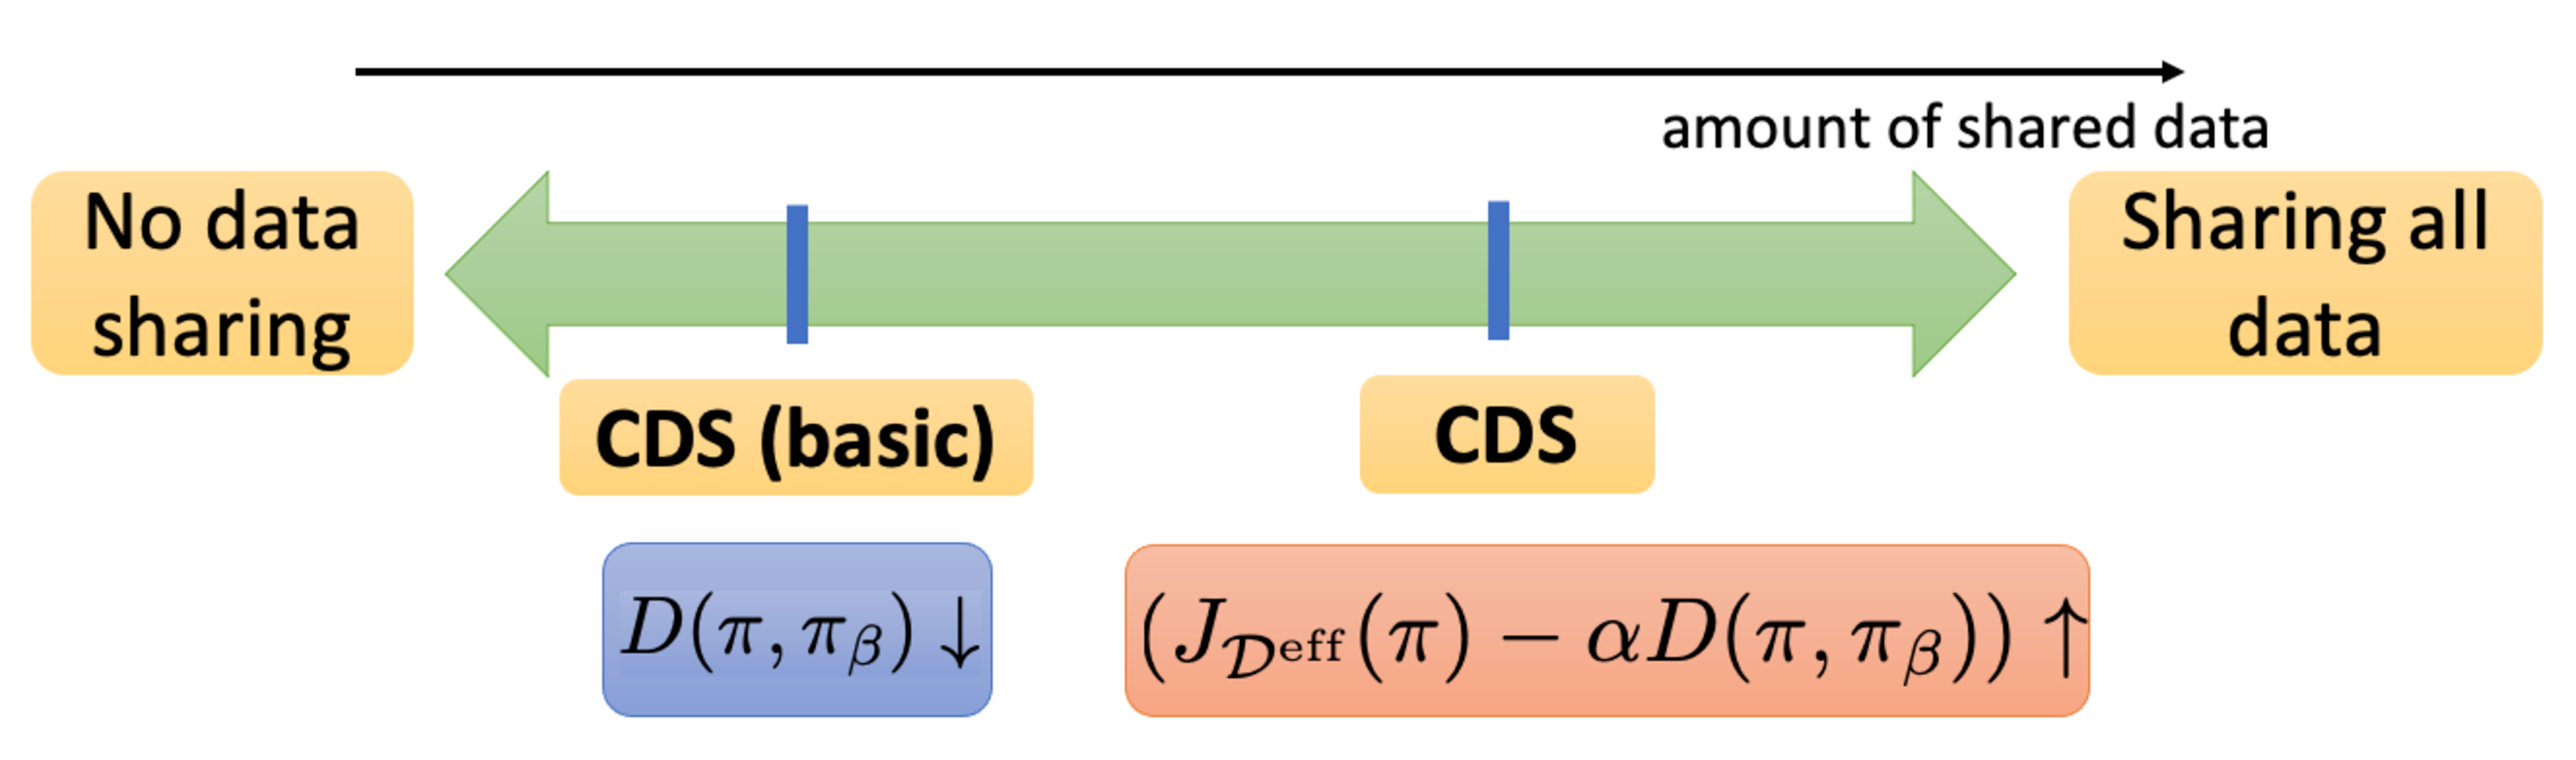
\includegraphics[width=0.99\linewidth]{chapters/cds/cds_variants.pdf}
%%CF.8.1: I think this is a nice figure. My only comment is that it isn't clear what "naive data sharing" means without having read parts of the main text. (and you should expect readers to skim figures without reading all of the text. I would change it to something like "Sharing all data" instead.
\vspace{-0.6cm}
\caption{\label{fig:cds_variants_main} \footnotesize A schematic comparing \textbf{CDS} and \textbf{CDS (basic)} data sharing schemes relative to no sharing (left extreme) and full data sharing (right extreme). While p-CDS only shares data when distributional shift is strictly reduced, o-CDS is more optimistic and shares data when the objective in Equation~\ref{eqn:generic_multitask_offline_rl} is larger. Typically, we would expect that CDS shares more transitions than CDS (basic).}
\vspace{-0.6cm}
\end{wrapfigure}
Next, we present the complete version of our method. The complete version of CDS, which we will refer to as \textbf{CDS}, for notational brevity is derived from the following perspective: we note that a data sharing scheme can be viewed as altering the dataset $\mathcal{D}^\mathrm{eff}_i$, and hence the effective behavior policy, $\pi^\mathrm{eff}_\beta(\mathbf{a}|\bs, i)$.
Thus, we can directly \emph{optimize} the objective in Equation~\ref{eqn:generic_multitask_offline_rl} with respect to $\pi^\mathrm{eff}_\beta$,
in addition to $\pi$, where $\pi^\mathrm{eff}_\beta$ belongs to the set of all possible effective behavior policies that can be obtained via any form of data sharing. Note that unlike CDS (basic), this approach would not rely on only indirectly controlling the objective in Equation~\ref{eqn:generic_multitask_offline_rl} by controlling distributional shift, but would aim to directly optimize the objective in Equation~\ref{eqn:generic_multitask_offline_rl}.  We formalize this optimization below in Equation~\ref{eqn:optimize_behavior}:
\begin{align}
\label{eqn:optimize_behavior}
    % &(\pi^*(\cdot|\cdot, i), \pi^\mathrm{eff}_\beta(\cdot|\cdot, i))\nonumber\\
    \arg \max_{\pi} \textcolor{red}{\max_{\pi^\mathrm{eff}_\beta \in \Pi_{\mathrm{relabel}}}}~~~ \left[J_{\mathcal{D}^\mathrm{eff}_i}(\pi) - \alpha D(\pi, \pi^\mathrm{eff}_\beta; i)\right],
\end{align}
where $\Pi_{\mathrm{relabel}}$ denotes the set of all possible behavior policies that can be obtained via relabeling. The next result characterizes safe policy improvement for Equation~\ref{eqn:optimize_behavior} and discusses how it leads to improvement over the behavior policy and also produces an effective practical method.

\begin{tcolorbox}[colback=blue!6!white,colframe=black,boxsep=0pt,top=-3pt,bottom=2pt]
\vspace{2mm}
\begin{proposition}[Characterizing safe-policy improvement for CDS.] 
\label{prop:spi_thm}
Let $\pi^*(\mathbf{a}|\bs)$ be the policy obtained from Equation~\ref{eqn:optimize_behavior}, and let $\pi_\beta(\mathbf{a}|\bs)$ be the behavior policy for $\mathcal{D}_i$. Then, w.h.p. $\geq 1 - \delta$, $\pi^*$ is a $\zeta$-safe policy improvement over $\pi_\beta$, i.e., $J(\pi^*) \geq J(\pi_\beta) - \zeta$, where $\zeta$ is given by:
\begin{align*}
\small{
    \!\!\zeta = \mathcal{O}\left(\frac{1}{(1 - \gamma)^2}\right)  \mathbb{E}_{\bs \sim d^{\pi^*}_{\mathcal{D}^\mathrm{eff}_i}}\left[\sqrt{\frac{D_{\text{CQL}}(\pi^*, \pi_\beta^*)(\bs) + 1}{|\mathcal{D}^\mathrm{eff}_i(\bs)|}} \right]
    -  \left[\alpha D(\pi^*, \pi_\beta^*) + \underbrace{J(\pi^*_\beta) - J(\pi_\beta)}_{\text{(a)}} \right],}
\end{align*}
\!\!where $\mathcal{D}^\mathrm{eff}_i \sim d^{\pi_\beta^*}(\bs)$ and $\pi^*_\beta(\mathbf{a}|\bs)$ denotes the policy $\pi \in \Pi_{\text{relabel}}$ that maximizes Equation~\ref{eqn:optimize_behavior}. 
\end{proposition}
\end{tcolorbox}
%%CF.8.1: I might consider putting this theoretical result back to the appendix. Right now, the main method doesn't come until the bottom of page 7, and the practical implementation doesn't come until page 8. Given that you can only really expect the reader to read ~9 pages, I think that the core info about the method is more important than this theoretical result.

A proof and analysis of this proposition is provided in Appendix~\ref{app:proofs}, where we note that the bound in Proposition~\ref{prop:spi_thm} is stronger than both no data sharing as well as na\"ive data sharing. We show in Appendix~\ref{app:proofs} that optimizing Equation~\ref{eqn:optimize_behavior} reduces the numerator $D_\mathrm{CQL}(\pi^*, \pi_\beta^*)$ term while also increasing $|\mathcal{D}^\mathrm{eff}_i(\bs)|$, thus reducing the amount of sampling error. In addition, Lemma~\ref{lemma:a_gt_0} shows that the improvement term $(a)$ is guaranteed to be positive if a large enough $\alpha$ is chosen in Equation~\ref{eqn:optimize_behavior}. Combining these, we find data sharing using Equation~\ref{eqn:optimize_behavior} improves over both complete data sharing (which may increase $D_\mathrm{CQL}(\pi, \pi_\beta)$) and no data sharing (which does not increase $|\mathcal{D}^\mathrm{eff}_i(\bs)|$). A schematic comparing the two variants of CDS and na\"ive and no data sharing schemes is shown in Figure~\ref{fig:cds_variants_main}.

~

\niparagraph{\textbf{Optimizing Equation~\ref{eqn:optimize_behavior} tractably.}} 
The next step is to effectively convert Equation~\ref{eqn:optimize_behavior} into a simple condition for data sharing in  multi-task offline RL. While directly solving Equation~\ref{eqn:optimize_behavior} is intractable in practice, since both the terms depend on $\pi^\mathrm{eff}_\beta(\mathbf{a}|\bs)$ (since the first term $J_{\mathcal{D}^\mathrm{eff}}(\pi)$ depends on the empirical MDP induced by the effective behavior policy and the amount of sampling error), we need to instead  solve Equation~\ref{eqn:optimize_behavior} approximately. Fortunately, we can optimize a \textit{lower-bound approximation} to Equation~\ref{eqn:optimize_behavior} that uses the dataset state distribution for the policy update in Equation~\ref{eqn:optimize_behavior} similar to modern actor-critic methods~\citep{degris2012off,lillicrap2015continuous,fujimoto2018addressing,haarnoja2018soft,kumar2020conservative} which only introduces an additional $D(\pi, \pi_\beta)$ term in the objective. This objective is given by: $\mathbb{E}_{\bs \sim \mathcal{D}^{\mathrm{eff}}_i}[\mathbb{E}_\pi[Q(\bs, \mathbf{a}, i)] - \alpha' D(\pi(\cdot|\bs,i), \pi_\beta^\mathrm{eff}(\cdot|\bs,i))]$, which is equal to the expected ``conservative Q-value'' $\hat{Q}^\pi(\bs, \mathbf{a}, i)$ on dataset states, policy actions and task $i$. Optimizing this objective via a co-ordinate descent on $\pi$ and $\pi^\mathrm{eff}_\beta$ dictates that $\pi$ be updated using a standard update of maximizing the conservative Q-function, $\hat{Q}^\pi$ (equal to the difference of the Q-function and $D(\pi, \pi^{\mathrm{eff}}_\beta; i)$).
Moreover, $\pi^{\mathrm{eff}}_\beta$ should also be updated towards maximizing the same expectation, $\mathbb{E}_{\bs, \mathbf{a} \sim \mathcal{D}^\mathrm{eff}_i}[\hat{Q}^\pi(\bs, \mathbf{a}, i)] := \mathbb{E}_{\bs, \mathbf{a} \sim \mathcal{D}^\mathrm{eff}_i}[Q(\bs, \mathbf{a}, i)] - \alpha D(\pi, \pi_\beta^\mathrm{eff}; i)$. This implies that when updating the behavior policy, we should prefer state-action pairs that maximize the conservative Q-function.
% Additionally $\pi^{\mathrm{eff}}_\beta$ should be updated towards minimizing the distribution shift $\mathbb{E}_{\bs, \mathbf{a} \sim \mathcal{D}^\mathrm{eff}_i}[ D(\pi, \pi_\beta^\mathrm{eff}; i)]$, i.e. learning a new behavior policy of task $i$ with minimal distribution shift after relabeling. In the case where $D(\pi, \pi_\beta^\mathrm{eff}; i) = D_\text{CQL}(\pi, \pi_\beta^\mathrm{eff}; i)$, we have the following objective for updating $\pi_\beta$: $\min_{\pi_\beta}\mathbb{E}_{\bs, \mathbf{a} \sim \mathcal{D}^\mathrm{eff}_i}[\hat{Q}^\pi(\bs,\mathbf{a}, i)]$
% \begin{align}
%     J_{\mathcal{D}^\mathrm{eff}_i}(\pi) - \alpha D(\pi, \pi^\mathrm{eff}_\beta; i) &:= \mathbb{E}_{\bs, \mathbf{a} \sim d^\pi_{\mathrm{eff}}}\left[Q(\bs, \mathbf{a}) - \alpha D(\pi, \pi_\right] 
% \end{align}

~

\niparagraph{\textbf{{Deriving the data sharing strategy for CDS.}}}
%%SL.8.1: not clear what the word "condition" means
%%CF.8.1: +1. What condition are you deriving?
%%AK: fixed
Utilizing the insights for optimizing Equation~\ref{eqn:optimize_behavior} tractably, we now present the effective data sharing rule prescribed by CDS. For any given task $i$, we want relabeling to incorporate transitions with the highest conservative Q-value into the resulting dataset $\mathcal{D}^\mathrm{eff}_i$, as this will directly optimize the tractable lower bound on Equation~\ref{eqn:optimize_behavior}. While directly optimizing Equation~\ref{eqn:optimize_behavior} will enjoy benefits of reduced sampling error since $J_{\mathcal{D}^\mathrm{eff}_i}(\pi)$ also depends on sampling error, our tractable lower bound approximation does not enjoy this benefit. This is because optimizing the lower-bound only increases the frequency of a state in the dataset, $|\mathcal{D}^\mathrm{eff}_i(\bs)|$ by atmost 1. To encourage further reduction in sampling error, we modify CDS to instead share all transitions with a conservative Q-value more than the top $k^\text{th}$ quantile of the original dataset $\mathcal{D}_i$, where $k$ is a hyperparameter. This provably increases the objective value in Equation~\ref{eqn:optimize_behavior} still ensuring that term $(a) > 0$ in Proposition~\ref{prop:spi_thm}, while also reducing $|\mathcal{D}^{\mathrm{eff}}_i(\bs)|$ in the denominator. Thus, for a given transition $(\bs, \mathbf{a}, \bs') \in \mathcal{D}_j$,  
\begin{tcolorbox}[colback=blue!6!white,colframe=black,boxsep=0pt,top=-5pt,bottom=5pt]
\begin{align}
   \text{\textbf{CDS}:~~~~~~~~} \!\!\!\!\!\!\!\!\!(\bs, \mathbf{a}, r_i, \bs') \in \mathcal{D}^{\mathrm{eff}}_i  \text{~if~} {\Delta}^\pi(\bs, \mathbf{a})\! := \hat{Q}^\pi(\bs, \mathbf{a}, i) - P_{k\%}\!\left\{\!\hat{Q}^\pi(\bs', \mathbf{a}', i)\!\!: \bs', \mathbf{a}' \sim \mathcal{D}_i\!\right\} \geq 0,
\label{eqn:method}
\end{align}
\end{tcolorbox}
where $\hat{Q}^\pi$ denotes the learned conservative Q-function estimate. If the condition in Equation~\ref{eqn:method} holds for the given $(\bs, \mathbf{a})$, then the corresponding relabeled transition, $(\bs, \mathbf{a}, r_{i}(\bs, \mathbf{a}), \bs')$ is added to $\mathcal{D}^\mathrm{eff}_i$. 

We summarize the pesudocode of CDS in Algorithm~\ref{alg:cds} in Appendix~\ref{app:alg} and include the practical implementation details of CDS in Appendix~\ref{app:details}.

% Our main data-sharing scheme, o-\cdsmethodname, is based on the insight discussed above. o-\cdsmethodname\ first runs any standard conservative offline RL algorithm on each task individually without any data sharing. Consistent with our insight from above, relabeling a transition that contributes a lower conservative Q-value to the current task will only decrease the average conservative Q-value of the effective resulting dataset for this task, whereas the $\pi^\mathrm{eff}_\beta$ is to be optimized to maximize this value. On the other hand, more samples in $\mathcal{D}^\mathrm{eff}_i$ will reduce sampling error. Hence, we employ a simple rule to decide which transitions from the data for other tasks will be relabeled to the current task, say task $i$: o-\cdsmethodname\ checks if the conservative Q-value estimate for this transition under task $i$ is greater than a specific percentile of the conservative Q-value for the original dataset for task $i$, $\mathcal{D}_i$. This is sufficient to increase the average conservative Q-value in $\mathcal{D}^\mathrm{eff}_i$ after relabeling, while still allowing us to keep sampling error under control.

% Thus, o-\cdsmethodname\ first estimates a conservative Q-value estimate, $\hat{Q}^\pi(\bs, \mathbf{a}, i)$ (which can be obtained via any offline RL algorithm), and for a given transition, $(\bs, \mathbf{a}, r_j, \bs') \in \mathcal{D}_j$ it then checks if the following condition is satisfied: 

% If the condition in Equation~\ref{eqn:method} holds for the given $(\bs, \mathbf{a})$, then the corresponding relabeled transition, $(\bs, \mathbf{a}, r_{i}(\bs, \mathbf{a}), \bs')$ is added to $\mathcal{D}^\mathrm{eff}_i$. \arxiv{In practice, instead of computing $\mathbb{E}_{\bs', \mathbf{a}' \sim \mathcal{D}_i}\left[ \hat{Q}^\pi(\bs', \mathbf{a}', i) \right]$, we use the $90$-th percentile of $\hat{Q}^\pi(\bs', \mathbf{a}', i)$ $\forall \bs', \mathbf{a}' \in \mathcal{D}_i$.} This rule for relabeling is applied independently on each transition $(\bs, \mathbf{a}, r, \bs') \in \mathcal{D}$. 

% \subsection{{Practical implementation of \cdsmethodname}} 
%%CF.8.1: In the section header and throughout the section, I would just have this discuss the main variant, not both. 
% The pseudocode of CDS is summarized in Algorithm~\ref{alg:cds} in Appendix~\ref{app:alg}. The complete variant of CDS can be directly implemented using the rule in Equation~\ref{eqn:method} with conservative Q-value estimates obtained via any offline RL method that constrains the learned policy to the behavior policy. For implementing \cdsmethodname\ (basic), we reparameterize the divergence $D$ in Equation~\ref{eqn:pessimistically_conservative} to use the learned conservative Q-values. This is especially useful for our implementation since we utilize CQL as the base offline RL method, and hence we do not have access to an explicit divergence. In this case, $\Delta^\pi(\bs, \mathbf{a})$ can be redefined as, $\Delta^\pi(\bs, \mathbf{a}) :=$
% \begin{align}
%     \mathbb{E}_{\bs' \sim \mathcal{D}^i}\left[\mathbb{E}_{\mathbf{a}' \sim \pi}[\hat{Q}(\bs', \mathbf{a}', i)] - \mathbb{E}_{\mathbf{a}'' \sim \mathcal{D}_i}[\hat{Q}(\bs', \mathbf{a}'', i)]\right] - \left(\mathbb{E}_{\mathbf{a}' \sim \pi}[\hat{Q}(\bs, \mathbf{a}', i)] - Q(\bs, \mathbf{a}, i)\right),
% \label{eqn:p-cds}
% \end{align}
% % \begin{align}
% %     \Delta^\pi(\bs, \mathbf{a})  := 
% %     -\left(\mathbb{E}_{\mathbf{a} \sim \mu(\cdot|\bs)}\!\left[Q(\bs,\mathbf{a}, i)\right]\!-\!\mathbb{E}_{\bs', \mathbf{a}' \sim \mathcal{D}_i}\!\left[Q(\bs',\mathbf{a}', i)\right]\right) +
% %     \left(\mathbb{E}_{\bs\sim \mathcal{D}_i, \mathbf{a} \sim \mu(\cdot|\bs)}\!\left[Q(\bs,\mathbf{a}, i)\right]\!-\!\mathbb{E}_{\bs', \mathbf{a}' \sim \mathcal{D}_i}\!\left[Q(\bs',\mathbf{a}', i)\right]\right)
% % \label{eqn:p-cds}
% % \end{align}
% % where $\mu(\cdot|s)$ is a wide sampling distribution such as the uniform distribution over the range of actions.
% Equation~\ref{eqn:p-cds} can be viewed as the difference between the CQL~\citep{kumar2020conservative} regularization term on a given $(\bs, \mathbf{a})$ and the original dataset for task $i$, $\mathcal{D}_i$. This CQL regularization term is equal to the divergence between the learned policy $\pi(\cdot|\bs)$ and the behavior policy $\pi_\beta(\cdot|\bs)$, therefore Equation~\ref{eqn:p-cds} practically computes Equation~\ref{eqn:pessimistically_conservative}. 
% % Intuitively, if the condition in Equation~\ref{eqn:p-cds} is true for certain $(\bs, \mathbf{a})$, adding it to $\mathcal{D}^\mathrm{eff}_i$ would decrease the expected CQL regularization term, which estimates the distributional shift $D_\text{CQL}(\pi(\cdot|\cdot, i), \pi_\beta^{\text{eff}}(\cdot|\cdot, i))$.

% Finally, both variants of \cdsmethodname\ train a policy, 
% $\pi(\mathbf{a}|\bs; i)$, either conditioned on the task $i$ (i.e., with weight sharing) or a separate $\pi(\mathbf{a}|\bs)$ policy for each task with no weight sharing, using the resulting relabeled dataset, $\mathcal{D}^\mathrm{eff}_i$.
% For practical implementation details of \cdsmethodname\, see Appendix~\ref{app:details}.

%%CF.5.22: you seem to have forgotten the punch line here.

%%SL.5.23: I think it would really help to add some pseudocode that describes the method. Right now, readers have to do a bit of detective work to piece together the complete algorithm. Pseudocode + algorithm summary would really help.

%%AK: just regular CQL weighted by the weights w_(s, a) described above

%%AK: there is a critical point here -- if we keep doing our scheme continually, would we eventually diverge, since we are doing many rounds of relabelling effectively? How should we handle that?



%% Theoretical Analysis

\section{Experimental Evaluation}
\label{sec:exp}

We conduct experiments to answer six main questions: \textbf{(1)} can \cdsmethodname\ prevent performance degradation when sharing data as observed in Section~\ref{sec:analysis}?, \textbf{(2)} how does \cdsmethodname\ compare to vanilla multi-task offline RL methods and prior data sharing methods?
\textbf{(3)} can \cdsmethodname\ handle sparse reward settings, where data sharing is particularly important due to scarce supervision signal? \textbf{(4)} can \cdsmethodname\ handle goal-conditioned offline RL settings where the offline dataset is undirected and highly suboptimal? \textbf{(5)} Can \cdsmethodname\ scale to complex visual observations? \arxiv{\textbf{(6)} Can \cdsmethodname\ be combined with any offline RL algorithms? Besides these questions, we visualize CDS weights for better interpretation of the data sharing scheme learned by CDS in Figure~\ref{fig:antmaze_vis} in Appendix~\ref{app:cds_vis}}.
%%CF.9.13: add or modify a question that includes how CDS combines with different algorithms?

%%AK.09.12: Need to fix the weird spacing issue here
\begin{wrapfigure}{r}{0.65\textwidth}
    \vspace{-0.65cm}
    \centering
    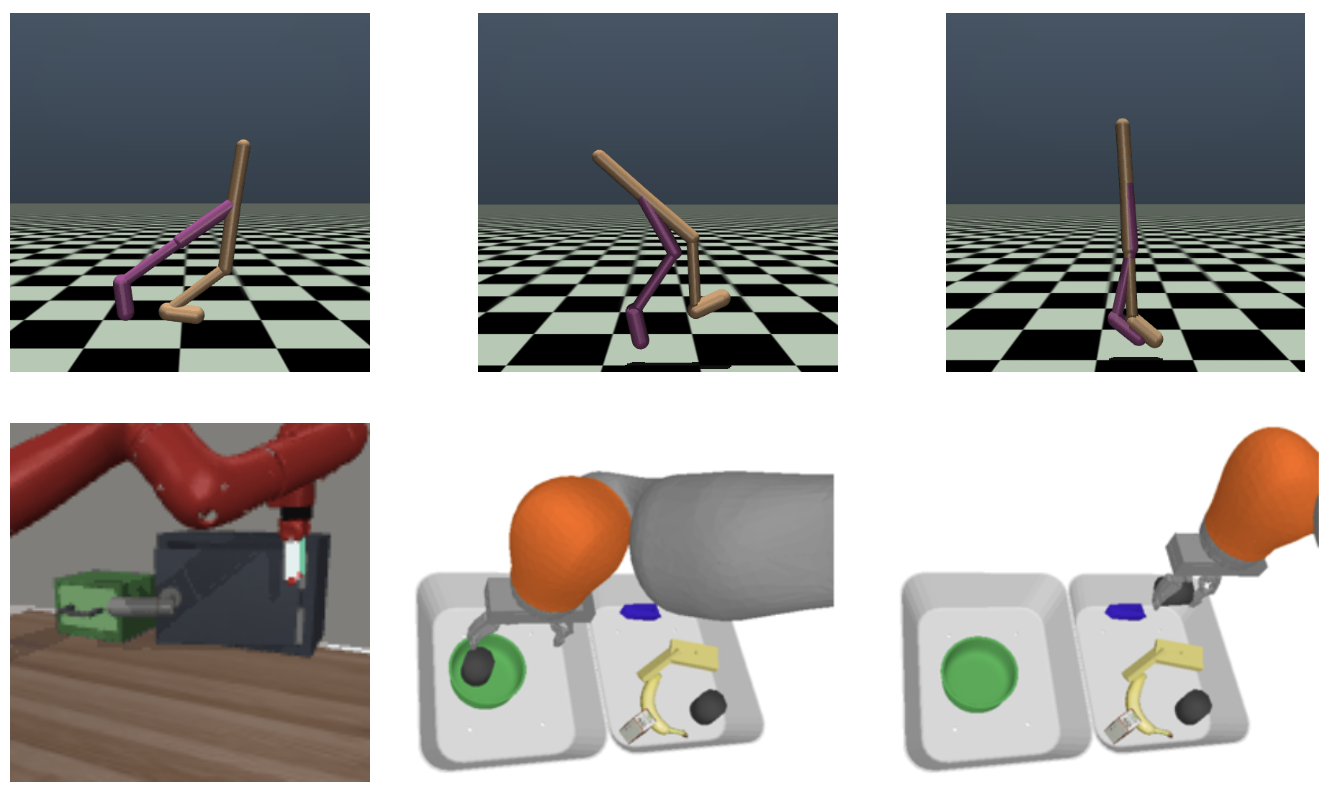
\includegraphics[width=0.61\textwidth]{chapters/cds/env.png}
    \vspace{-0.32cm}
    \caption{\footnotesize  Environments (from left to right): walker2d {run forward}, walker2d {run backward}, walker2d {jump},  Meta-World {door open/close} and {drawer open/close} and vision-based pick-place tasks in \citep{kalashnikov2021mt}.}
    \label{fig:env}
    \vspace{-0.4cm}
\end{wrapfigure}
\textbf{Comparisons.} To answer these questions, we consider the following prior methods. On tasks with low dimensional state spaces, we compare with the online multi-task relabeling approach \textbf{HIPI}~\citep{eysenbach2020rewriting}, which uses inverse RL to infer for which tasks the datapoints are optimal and in practice routes a transition to task with the highest Q-value. We adapt HIPI to the offline setting by applying its data routing strategy to a conservative offline RL algorithm.
We also compare to na\"ively sharing data across all tasks (denoted as \textbf{Sharing All}) and vanilla multi-task offline RL method without any data sharing (denoted as \textbf{No Sharing}). On image-based domains, we compare \cdsmethodname\ to the data sharing strategy based on human-defined skills~\citep{kalashnikov2021mt} (denoted as \textbf{Skill}), which manually groups tasks into different skills (e.g. skill ``pick'' and skill ``place'') and only routes an episode to target tasks that belongs to the same skill.
In these domains, we also compare to \textbf{HIPI}, \textbf{Sharing All} and \textbf{No Sharing}. \arxiv{Beyond these multi-task RL approaches with data sharing, to assess the importance of data sharing in offline RL, we perform an additional comparison to other alternatives to data sharing in multi-task offline RL settings. One traditionally considered approach is to use data from other tasks for some form of ``pre-training'' before learning to solve the actual task. We instantiate this idea by considering a method from \citet{yang2021representation} that conducts contrastive representation learning on the multi-task datasets to extract shared representation between tasks and then runs multi-task RL on the learned representations. We discuss this comparison in detail in Table~\ref{tbl:pretrain_comparison} in Appendix~\ref{app:pretrain_comparison}.} 
%%CF.9.13: It's not at all clear why the above comparison is informative/useful.
%%KY.9.13: added such discussion.
%%CF.9.13: I would combine the next two sentences. You do not use CQL for all methods because some experiments use BRAC.
%%KY.9.13: done.
To answer question (6), we use CQL~\citep{kumar2020conservative} (a Q-function regularization method) and BRAC~\citep{wu2019behavior} (a policy-constraint method) as the base offline RL algorithms for all methods. \arxiv{We discuss evaluations of CDS with CQL in the main text and include the results of CDS with BRAC in Table~\ref{tbl:brac_comparison} in Appendix~\ref{app:brac_results}.} 
%%CF.9.13: the visualization of the weights is not a comparison (the paragraph header). I would put this sentence somewhere else more appropriate, maybe in one of the results sections or right after you list the questions.
%%KY.9.13: moved it to the end of the first para of the section right after the list the questions.
For more details on setup and hyperparameters, see Appendix~\ref{app:details}.

% \subsection{Results on domains with low-dimensional inputs}
% \label{sec:gym_results}

\textbf{Multi-task environments.} We consider a number of multi-task reinforcement learning problems on environments visualized in Figure~\ref{fig:env}. 
% To answer questions (1) and (2), we consider three locomotion environments from OpenAI Gym~\citep{brockman2016openai} with dense rewards: halfcheetah, walker2d, and ant. Each environment has three tasks, \texttt{run forward}, \texttt{run backward} and \texttt{jump}, as used in prior offline RL work~\citep{yu2020mopo}.
\arxiv{To answer questions (1) and (2), we consider the walker2d locomotion environment from OpenAI Gym~\citep{brockman2016openai} with dense rewards. We use three tasks, \texttt{run forward}, \texttt{run backward} and \texttt{jump}, as proposed in prior offline RL work~\citep{yu2020mopo}.}
To answer question (3), we also evaluate on robotic manipulation domains using environments from the Meta-World benchmark~\citep{yu2020metaworld}. We consider four tasks: \texttt{door open}, \texttt{door close}, \texttt{drawer open} and \texttt{drawer close}. Meaningful data sharing requires a consistent state representation across tasks, so we put both the door and the drawer on the same table, as shown in Figure~\ref{fig:env}. Each task has a sparse reward of 1 when the success condition is met and 0 otherwise. To answer question (4), we consider maze navigation tasks where the temporal ``stitching'' ability of an offline RL algorithm is crucial to obtain good performance. We create goal reaching tasks using the ant robot in the medium and hard mazes from D4RL~\citep{fu2020d4rl}. The set of goals is a fixed discrete set of size 7 and 3 for large and medium mazes, respectively. Following \citet{fu2020d4rl}, a reward of +1 is given and the episode terminates if the state is within a threshold radius of the goal. Finally, to explore how \cdsmethodname\ scales to image-based manipulation tasks (question (5)), we utilize a simulation environment similar to the real-world setup presented in~\citep{kalashnikov2021mt}. This environment, which was utilized by \citet{kalashnikov2021mt} as a representative and realistic simulation of a real-world robotic manipulation problem, consists of 10 image-based manipulation tasks that involve different combinations of picking specific objects (banana, bottle, sausage, milk box, food box, can and carrot) and placing them in one of the three fixtures (bowl, plate and divider plate) (see example task images in Fig.~\ref{fig:env}).
More environment details are in the appendix. We report the average return for locomotion tasks and success rate for AntMaze and both manipluation environments, averaged over 6 and 3 random seeds for environments with low-dimensional inputs and image inputs respectively.

\begin{table}[h]
\vspace{0.1cm}
  \centering
  \scriptsize
  \def\arraystretch{0.9}
  \setlength{\tabcolsep}{0.42em}
  \vspace{-0.4cm}
\begin{tabularx}{0.75\linewidth}{cc|cccc}
  \toprule
 \multicolumn{1}{c}{\multirow{1.5}[2]{*}{Environment}} & \multicolumn{1}{c}{\multirow{1.5}[2]{*}{Dataset types / Tasks}}\vline &
 \multicolumn{3}{c}{$D_\text{KL}(\pi, \pi_\beta)$}\\
& \multicolumn{1}{c}{} \vline& \multicolumn{1}{c}{\textbf{No Sharing}}  & \multicolumn{1}{c}{\textbf{Sharing All}} & \multicolumn{1}{c}{\textbf{CDS (basic) (ours)}}  & \multicolumn{1}{c}{\textbf{CDS (ours)}}\\
\midrule
  &medium-replay / run forward & \textbf{1.49} & 7.76 & 14.31 & \textbf{1.49}\\
  walker2d& medium / run backward &  \textbf{1.91} & 12.2 & 8.26 & 6.09\\
  %\rowcolor{Gray}
  & \cellcolor{yellow} expert / jump & \cellcolor{yellow} 3.12 & \cellcolor{yellow} 27.5 & \cellcolor{yellow} 13.25  & \cellcolor{yellow} \textbf{2.91}\\
    \bottomrule
    \end{tabularx}
    \vspace{0.1cm}
         \caption{\footnotesize Measuring $D_\text{KL}(\pi, \pi_\beta)$ on the walker2d environment.  \textbf{Sharing All} degrades the performance on task \text{jump} with limited expert data as discussed in Table~\ref{tab:analysis}. \cdsmethodname\ manages to obtain a $\behavior$ after data sharing that is closer to the single-task optimal policy in terms of the KL divergence compared to \textbf{No Sharing} and \textbf{Sharing All} on task \texttt{jump} (highlighted in yellow). Since \cdsmethodname\ also achieves better performance, this analysis suggests that reducing distribution shift is important for effective offline data sharing.
     \label{tab:analysis_cds}
     \vspace{-0.5cm}
     }
\end{table}

\textbf{Multi-task datasets.}  Following the analysis in Section~\ref{sec:analysis}, we intentionally construct datasets with a variety of heterogeneous behavior policies to test if \cdsmethodname\ can provide effective data sharing to improve performance while avoiding harmful data sharing that exacerbates distributional shift. For the locomotion domain, we use a large, diverse dataset (medium-replay) for \texttt{run forward}, a medium-sized dataset for \texttt{run backward}, and an expert dataset with limited data for \texttt{run jump}. For Meta-World, we consider medium-replay datasets with 152K transitions for task \texttt{door close} and \texttt{drawer open} and expert datasets with only 2K transitions for task \texttt{door open} and \texttt{drawer close}. For AntMaze, we modify the D4RL datasets for antmaze-*-play environments to construct two kinds of multi-task datasets: an ``undirected'' dataset, where data is equally divided between different tasks and the rewards are correspondingly relabeled, and a ``directed'' dataset, where a trajectory is associated with the goal closest to the final state of the trajectory. This means that the per-task data in the undirected setting may not be relevant to reaching the goal of interest. Thus, data-sharing is crucial for good performance: methods that do not effectively perform data sharing and train on largely task-irrelevant data are expected to perform worse. Finally, for image-based manipulation tasks, we collect datasets for all the tasks individually by running online RL~\cite{kalashnikov2018scalable} until the task reaches medium-level performance (40\% for picking tasks and 80\% placing tasks). At that point, we merge the entire replay buffers from different tasks creating a final dataset of 100K RL episodes with 25 transitions for each episode.

\begin{table*}[t!]
\centering
\vspace*{0.1cm}
\scriptsize
\resizebox{\textwidth}{!}{\begin{tabular}{l|l|r|r|r|r|r}
\toprule
\textbf{Environment} & \textbf{Tasks / Dataset type} & \textbf{\cdsmethodname\ (ours)} & \textbf{\cdsmethodname\ (basic)} & \textbf{HIPI}~\cite{eysenbach2020rewriting}& \textbf{Sharing All} & \textbf{No Sharing}\\ \midrule
% & run forward / medium-replay & 2587.7  & \textbf{2626.1} & 2605.0 & \textbf{2632.5}\\
% halfcheetah & run backward / medium & 2519.5  & \textbf{2634.4} & \textbf{2636.7} & \textbf{2630.7}\\
% & jump / expert & \textbf{4298.2} & 4113.4 & 712.3 & -1978.3\\
% & \CC \textbf{average} & \CC \textbf{3135.1} & \CC \textbf{3124.7} & \CC 1984.7 & \CC 1095.0\\
% \midrule
& run forward / medium-replay & \textbf{1057.9}$\pm$121.6 & 968.6$\pm$188.6 & 695.5$\pm$61.9 & 701.4$\pm$47.0 & 590.1$\pm$48.6\\
walker2d & run backward / medium & 564.8$\pm$47.7 & 594.5$\pm$22.7 & 626.0$\pm$48.0& \textbf{756.7}$\pm$76.7& 614.7$\pm$87.3\\
& jump / expert & 1418.2$\pm$138.4 & 1501.8$\pm$115.1  & \textbf{1603.7}$\pm$146.8 & 885.1$\pm$152.9 & 1575.2$\pm$70.9\\
& \CC \textbf{average} & \CC 1013.6$\pm$71.5 &\CC \textbf{1021.6}$\pm$76.9 & \CC 975.1$\pm$45.1 & \CC 781.0$\pm$100.8 & \CC 926.6$\pm$37.7\\\midrule
% & run forward / medium-replay & 2350.1 & \textbf{2658.9} & 1175.0 & 2126.7\\
% ant & run backward / medium & 1435.7 & 1208.2 & 1488.7 & \textbf{2021.7}\\
% & jump / expert & \textbf{2781.3} & 2670.4 & 133.8 & 495.8\\
% & \CC \textbf{average} & \CC \textbf{2189.0} & \CC \textbf{2179.2} & \CC 932.5 & \CC 1548.1\\
% \midrule
& door open / expert & \textbf{58.4\%}$\pm$9.3\% & 30.1\%$\pm$16.6\% & 26.5\%$\pm$20.5\% & 34.3\%$\pm$17.9\% & 14.5\%$\pm$12.7\\
& door close / medium-replay & \textbf{65.3\%}$\pm$27.7\% & 41.5\%$\pm$28.2\% & 1.3\%$\pm$5.3\% & 48.3\%$\pm$27.3\% & 4.0\%$\pm$6.1\% \\
Meta-World~\citep{yu2020metaworld}& drawer open / medium-replay & \textbf{57.9\%}$\pm$16.2\% & 39.4\%$\pm$16.9\% & 41.2\%$\pm$24.9\% & 55.1\%$\pm$9.4\% & 16.0\%$\pm$17.5\%\\
& drawer close / expert & 98.8\%$\pm$0.7\% & 86.3\%$\pm$0.9\% & 62.2\%$\pm$33.4\% & \textbf{100.0\%}$\pm$0\% & 99.0\%$\pm$0.7\%\\
& \CC \textbf{average} & \CC \textbf{70.1\%}$\pm$8.1\% & \CC 49.3\%$\pm$16.0\% & \CC 32.8\%$\pm$18.7\% & \CC 59.4\%$\pm$5.7\% & \CC 33.4\%$\pm$8.3\%\\
\midrule
& large maze (7 tasks) / undirected & \textbf{22.8}\% $\pm$ 4.5\% & 10.0\% $\pm$ 5.9\% & 1.3\% $\pm$ 2.3\%  & 16.7\% $\pm$ 7.0\% & 13.3\% $\pm$ 8.6\% \\
AntMaze~\citep{fu2020d4rl}  & large maze (7 tasks) / directed &  \textbf{24.6\%} $\pm$ 4.7\% & 0.0\% $\pm$ 0.0\% & 11.8\% $\pm$ 5.4\% & 20.6\% $\pm$ 4.4\% & 19.2\% $\pm$ 8.0\% \\
& medium maze (3 tasks) / undirected &  \textbf{36.7\%} $\pm$ 6.2\% & 0.0\% $\pm$ 0.0\% & 8.6\% $\pm$ 3.2\% & 22.9\% $\pm$ 3.6\% & 21.6\% $\pm$ 7.1\% \\
& medium maze (3 tasks) / directed &  \textbf{18.5}\% $\pm$ 6.0\% & 0.0\% $\pm$ 0.0\% & 8.3\% $\pm$ 9.1\% & 12.4\% $\pm$ 5.4\% & \textbf{17.0\%} $\pm$ 3.2\% \\
\bottomrule
\end{tabular}}
\vspace{-0.2cm}
\caption{\footnotesize Results for multi-task locomotion (walker2d), robotic manipulation (Meta-World) and navigation environments (AntMaze) with low-dimensional state inputs.
% On the locomotion environment walker2d, we include three tasks with different styles of datasets, \texttt{run forward} + a medium replay dataset, \texttt{run backward} + a medium dataset and \texttt{jump} + an expert dataset with limited data. On the multi-task robotic manipulation domain, we consider four tasks from Meta-World~\citep{yu2020metaworld}, door open, door close, drawer open and drawer close with medium-replay, expert, medium-replay and expert datasets respectively.
% % Similar to locomotion tasks, we also used limited amount of expert trajectories for the expert dataset.
% On the antmaze navigation task, we consider two maze layouts (medium/large) from D4RL~\citep{fu2020d4rl} with the directed and undirected datasets.
 \arxiv{Numbers are averaged across 6 seeds, $\pm$ the 95$\%$-confidence interval.} We include per-task performance for walker2d and Meta-World domains and the overall performance averaged across tasks (highlighted in gray) for all three domains. We bold the highest score across all methods. \cdsmethodname\ achieves the best or comparable performance on all of these environments.
}
\label{tbl:gym}
\normalsize
\vspace{-0.3cm}
\end{table*}
%%AK: things seemed a bit diverging with CDS (basic) on antmaze, I guess it is fine for now since it is not the main method, but we could revisit back later during camera-ready.

\begin{table*}[t!]
\small{
\centering
\vspace*{0.1cm}
\resizebox{\textwidth}{!}{\begin{tabular}{l|r|r|r|r|r}
\toprule
\textbf{Task Name} & \textbf{\cdsmethodname\ (ours)}& \textbf{HIPI}~\cite{eysenbach2020rewriting} & \textbf{Skill~\cite{kalashnikov2021mt}} & \textbf{Sharing All} & \textbf{No Sharing}\\ \midrule
\texttt{lift-banana} & \textbf{53.1\%}$\pm$3.2\% & 48.3\%$\pm$6.0\%  & 32.1\%$\pm$9.5\% & 41.8\%$\pm$4.2\% & 20.0\%$\pm$6.0\%\\
\texttt{lift-bottle} & \textbf{74.0\%}$\pm$6.3\% & 64.4\%$\pm$7.7\%  & 55.9\%$\pm$9.6\% & 60.1\%$\pm$10.2\% & 49.7\%$\pm$8.7\%\\
\texttt{lift-sausage} & \textbf{71.8\%}$\pm$3.9\%  & 71.0\%$\pm$7.7\%  & 68.8\%$\pm$9.3\% & 70.0\%$\pm$7.0\% & 60.9\%$\pm$6.6\%\\
\texttt{lift-milk}& \textbf{83.4\%}$\pm$5.2\% & 79.0\%$\pm$3.9\% & 68.2\%$\pm$3.5\% & 72.5\%$\pm$5.3\% & 68.4\%$\pm$6.1\%\\

\texttt{lift-food} & 61.4\%$\pm$9.5\% & \textbf{62.6\%}$\pm$6.3\% & 41.5\%$\pm$12.1\% & 58.5\%$\pm$7.0\% & 39.1\%$\pm$7.0\%\\
\texttt{lift-can} & 65.5\%$\pm$6.9\% & \textbf{67.8\%}$\pm$6.8\%  & 50.8\%$\pm$12.5\% & 57.7\%$\pm$7.2\% & 49.1\%$\pm$9.8\%\\
\texttt{lift-carrot} & \textbf{83.8\%}$\pm$3.5\% & 78.8\%$\pm$6.9\% & 66.0\%$\pm$7.0\%& 75.2\%$\pm$7.6\%& 69.4\%$\pm$7.6\%\\
\texttt{place-bowl} & \textbf{81.0\%}$\pm$8.1\%  & 77.2\%$\pm$8.9\% & 80.8\%$\pm$6.9\% & 70.8\%$\pm$7.8\% & 80.3\%$\pm$8.6\%\\
\texttt{place-plate} & 85.8\%$\pm$6.6\%  & 83.6\%$\pm$7.9\% & 78.4\%$\pm$9.6\% & 78.7\%$\pm$7.6\% & \textbf{86.1}\%$\pm$7.7\%\\
\texttt{place-divider-plate} & \textbf{87.8\%}$\pm$7.6\%  & 78.0\%$\pm$10.5\% & 80.8\%$\pm$5.3\% & 79.2\%$\pm$6.3\% & 85.0\%$\pm$5.9\%\\
%\midrule
\CC \textbf{average} & \CC \textbf{74.8\%}$\pm$6.4\%  & \CC 71.1\%$\pm$7.5\% & \CC 62.3\%$\pm$8.9\% & \CC 66.4\%$\pm$7.2\% & \CC 60.8\%$\pm$7.5\%\\
\bottomrule
\end{tabular}}
\vspace{-0.1cm}
\caption{\footnotesize Results for multi-task vision-based robotic manipulation domains in \citep{kalashnikov2021mt}. \arxiv{Numbers are averaged across 3 seeds, $\pm$ the 95$\%$ confidence interval.} We consider 7 tasks denoted as \texttt{lift-object} where the goal of each task is to lift a different object and 3 tasks denoted as \texttt{place-fixture} that aim to place a lifted object onto different fixtures. \cdsmethodname\ outperforms both a skill-based data sharing strategy~\citep{kalashnikov2021mt} (\textbf{Skill}) and other data sharing methods on the average task success rate (highlighted in gray) and 7 out of 10 per-task success rates.
}
\label{tbl:mtopt}
}
\vspace{-0.6cm}
\end{table*}


% \subsection{Evaluating CDS on Multi-Task Offline RL}
\textbf{Results on domains with low-dimensional states.} We present the results on all non-vision environments in Table~\ref{tbl:gym}.
% , but leave the results of halfcheetah and ant to Appendix~\ref{app:additional_exp}. 
\cdsmethodname\ achieves the 
best average performance across all environments except that on walker2d, it achieves the second best performance, obtaining slightly worse the other variant \cdsmethodname\ (basic). On the locomotion domain, we observe the most 
significant improvement on task \texttt{jump} on all three environments. We interpret this as strength of conservative data sharing, which mitigates the distribution shift that can be introduced by routing large amount of other task data to the task with limited data and narrow distribution. We also validate this by measuring the $D_\text{KL}(\pi, \pi_\beta)$ in Table~\ref{tab:analysis_cds} where $\pi_\beta$ is the behavior policy after we perform \cdsmethodname\
to share data. As shown in Table~\ref{tab:analysis_cds}, \cdsmethodname\ achieves lower KL divergence
 between the single-task optimal policy and the behavior policy after data sharing on task \texttt{jump} with limited expert data, whereas \textbf{Sharing All} results in much higher KL divergence compared to \textbf{No Sharing} as discussed in Section~\ref{sec:analysis} and Table~\ref{tab:analysis}. Hence, \cdsmethodname\ is able to mitigate distribution shift when sharing data and result in performance boost.


On the Meta-World tasks, we find that the agent without data sharing completely fails to solve most of the tasks due to the low quality of the medium replay datasets and the insufficient data for the expert datasets. \textbf{Sharing All} improves performance since in the sparse reward settings, data sharing can introduce more supervision signal and help training. \cdsmethodname\ further improves over \textbf{Sharing All}, suggesting that \cdsmethodname\ can not only prevent harmful data sharing, but also lead to more effective multi-task learning compared to \textbf{Sharing All} in scenarios where data sharing is imperative. It's worth noting that \cdsmethodname\ (basic) performs worse than \cdsmethodname\ and \textbf{Sharing All}, indicating that relabeling data that only mitigates distributional shift is too pessimistic and might not be sufficient to discover the shared structure across tasks.

%\textbf{Goal-conditioned AntMazes~\citep{fu2020d4rl}.} 

In the AntMaze tasks, we observe that \cdsmethodname\ performs better than \textbf{Sharing All} and significantly outperforms HIPI in all four settings. Perhaps surprisingly, \textbf{No Sharing} is a strong baseline, however, is outperformed by \cdsmethodname\ with the harder undirected data. Moreover, \cdsmethodname\ performs on-par or better in the undirected setting compared to the directed setting, indicating the effectiveness of \cdsmethodname\ in routing data in challenging settings. 




% Concretely, we consider three different styles of datasets in gym domains: medium-replay for \texttt{run forward}, medium for \texttt{run backward}, and expert for \texttt{run jump}, following the convention proposed in \citep{fu2020d4rl}.

% Since it is common to generate a large number of data from multiple policies with different levels of performance, we use 120K, 120K and 250K datapoints 
% %%CF.5.22: are you referring to different checkpoints or different #s of datapoints?
% %%TY.5.26: I mean different number of datapoints.
% medium-replay datasets in halfcheetah, walker2d and ant respectively. Meanwhile, it is usually time-consuming to collect medium or high quality data in the real world and thus we provide 25K, 25K and 50K datapoints for medium datasets and 5K, 5K and 20K datapoints for expert datasets for the aforementioned three environments respectively.
% As analyzed in Section~\ref{sec:analysis} and Table~\ref{tab:analysis}, na\"ively sharing data across all tasks would hurt multi-task performance when behavior policies differ in each task. To test if \cdsmethodname\ can mitigate this issue, we adopt medium-replay datasets for task \texttt{run forward}, medium datasets for task \texttt{run backward} and expert datasets for task \texttt{jump}.










% \subsection{Results on image-based robotic manipulation tasks}
% \label{sec:mtopt_results}

\textbf{Results on image-based robotic manipulation domains.}  %\textbf{Skill} manually defines two oracle skills ``picking'' and ``placing'' and shares all picking tasks share data with each other but does not share data with any of the placing tasks and vice-versa. 
Here, we compare \cdsmethodname\ to the hand-designed \textbf{Skill} sharing strategy, in addition to the other methods. \arxiv{Given that \cdsmethodname\ achieves significantly better performance than \cdsmethodname\ (basic) on low-dimensional robotic manipulation tasks in Meta-World, we only evaluate \cdsmethodname\ in the vision-based robotic manipulation domains.}  Since \cdsmethodname\ is applicable to any offline multi-task RL algorithm, we employ it as a separate data-sharing strategy in \citep{kalashnikov2021mt} while keeping the model architecture and all the other hyperparameters constant, which allows us to carefully evaluate the influence of data sharing in isolation. The results are reported in Table~\ref{tbl:mtopt}. \cdsmethodname\ outperforms both \textbf{Skill} and other approaches, indicating that \cdsmethodname\ is able to scale to high-dimensional observation inputs and can effectively remove the need for manual curation of data sharing strategies.


    
% \section{Discussion and Perspectives}
% \label{sec:conclusion}
% In this paper, we study the multi-task offline RL setting, focusing on the problem of sharing offline data across tasks for better multi-task learning. Through empirical analysis, we identify that na\"{i}vely sharing data across tasks generally helps learning but can significantly hurt performance in scenarios where excessive distribution shift is introduced. To address this challenge, we present conservative data sharing (CDS), which relabels data to a task when the conservative Q-value of the given transition is better than the expected conservative Q-value of the target task. On multitask locomotion, manipulation, navigation, and vision-based manipulation domains, CDS consistently outperforms or achieves comparable performance to existing data sharing approaches. While CDS attains superior results, it is not able to handle data sharing in settings where dynamics vary across tasks and requires functional forms of rewards. We leave these as future work. 
% Another limitation of CDS is that it requires access to the functional form of the reward. Though this is a common assumption as discussed in Section~\ref{sec:prelims}, an interesting future direction would be removing this dependence and replacing it with either a learned reward predictor or other supervision signal like language instructions.
    

%%%%%%%%%%%%%%%%%%%%%%%%%%%%%%%%%%%%%%%%%%%%%%%%%%%%%%%%%%%%%%%%%%%%%%%%%%%%%%%%%%%%%%%%%%%%%%%%%
%%%%%%%%%%%%%%%%%%%%%%%%%%%%%%%%%%       UDS      %%%%%%%%%%%%%%%%%%%%%%%%%%%%%%%%%%%%%%%%%%%%%%%
%%%%%%%%%%%%%%%%%%%%%%%%%%%%%%%%%%%%%%%%%%%%%%%%%%%%%%%%%%%%%%%%%%%%%%%%%%%%%%%%%%%%%%%%%%%%%%%%%

\vspace{-0.2cm}
\section{Multi-Task Offline RL With Unlabeled Data}
\label{sec:uds_section}
\vspace{-0.2cm}

% \section{Introduction}
% Offline reinforcement learning (RL) provides the promise of a fully data-driven framework for learning performant policies. To avoid costly active data collection and exploration, offline RL methods utilize a previously collected dataset to extract the best possible behavior, making it feasible to use RL to solve real-world problems where active exploration is expensive, dangerous, or otherwise infeasible~\citep{zhan2021deepthermal, de2021discovering, Wang2018SupervisedRL, kalashnikov2018scalable}. 
% However, this concept is only viable when a significant amount of data for the target task is available in advance. A more realistic scenario might allow for a much smaller amount of task-specific data, combined with a large amount of task-agnostic data, that is not labeled with task rewards and some of which may not be relevant. For example, if our goal is to train a robot to perform a new manipulation task (e.g., cutting an onion), we might have some data of the robot (suboptimally) attempting that task, perhaps collected under human teleoperation and manually labeled with rewards, combined with background data, some of which might be structurally related (e.g., picking up an onion, or cutting a carrot). {This scenario presents several questions: How do we decide which prior data should be included when learning the new task? And how do we determine reward labels to use for this prior data?}

% Prior methods have attempted to answer these two questions, typically in isolation. For the first question, it has been noted that a na\"{i}ve strategy of sharing all of the prior data can be highly suboptimal~\citep{kalashnikov2021mt}, even when it is annotated with reward labels, and some works have proposed both manual~\citep{kalashnikov2021mt} and automated~\citep{yu2021conservative,eysenbach2020rewriting} data sharing strategies that prioritize the most structurally similar prior data. 
% However, these methods assume that shared data can automatically be relabeled with the reward function for the task,
% but the assumption that we have access to the functional form of this reward is a strong one: for example, in many real-world settings, computing the reward might require human labeling~\citep{cabi2019scaling,finn2016deep}. 
% Prior works use learned classifiers for reward labeling~\citep{VICEFu2018,xie2018few,singh2019end}, or other automated mechanisms~\citep{konyushkova2020semi}. But these mechanisms themselves add complexity and potential brittleness to the pipeline. Thus, we aim to study the possibility of tackling this problem with a simple method that determines which rewards to use for shared data, with minimal supervision and no additional modeling and learning.

\begin{figure}[ht]
    \centering
    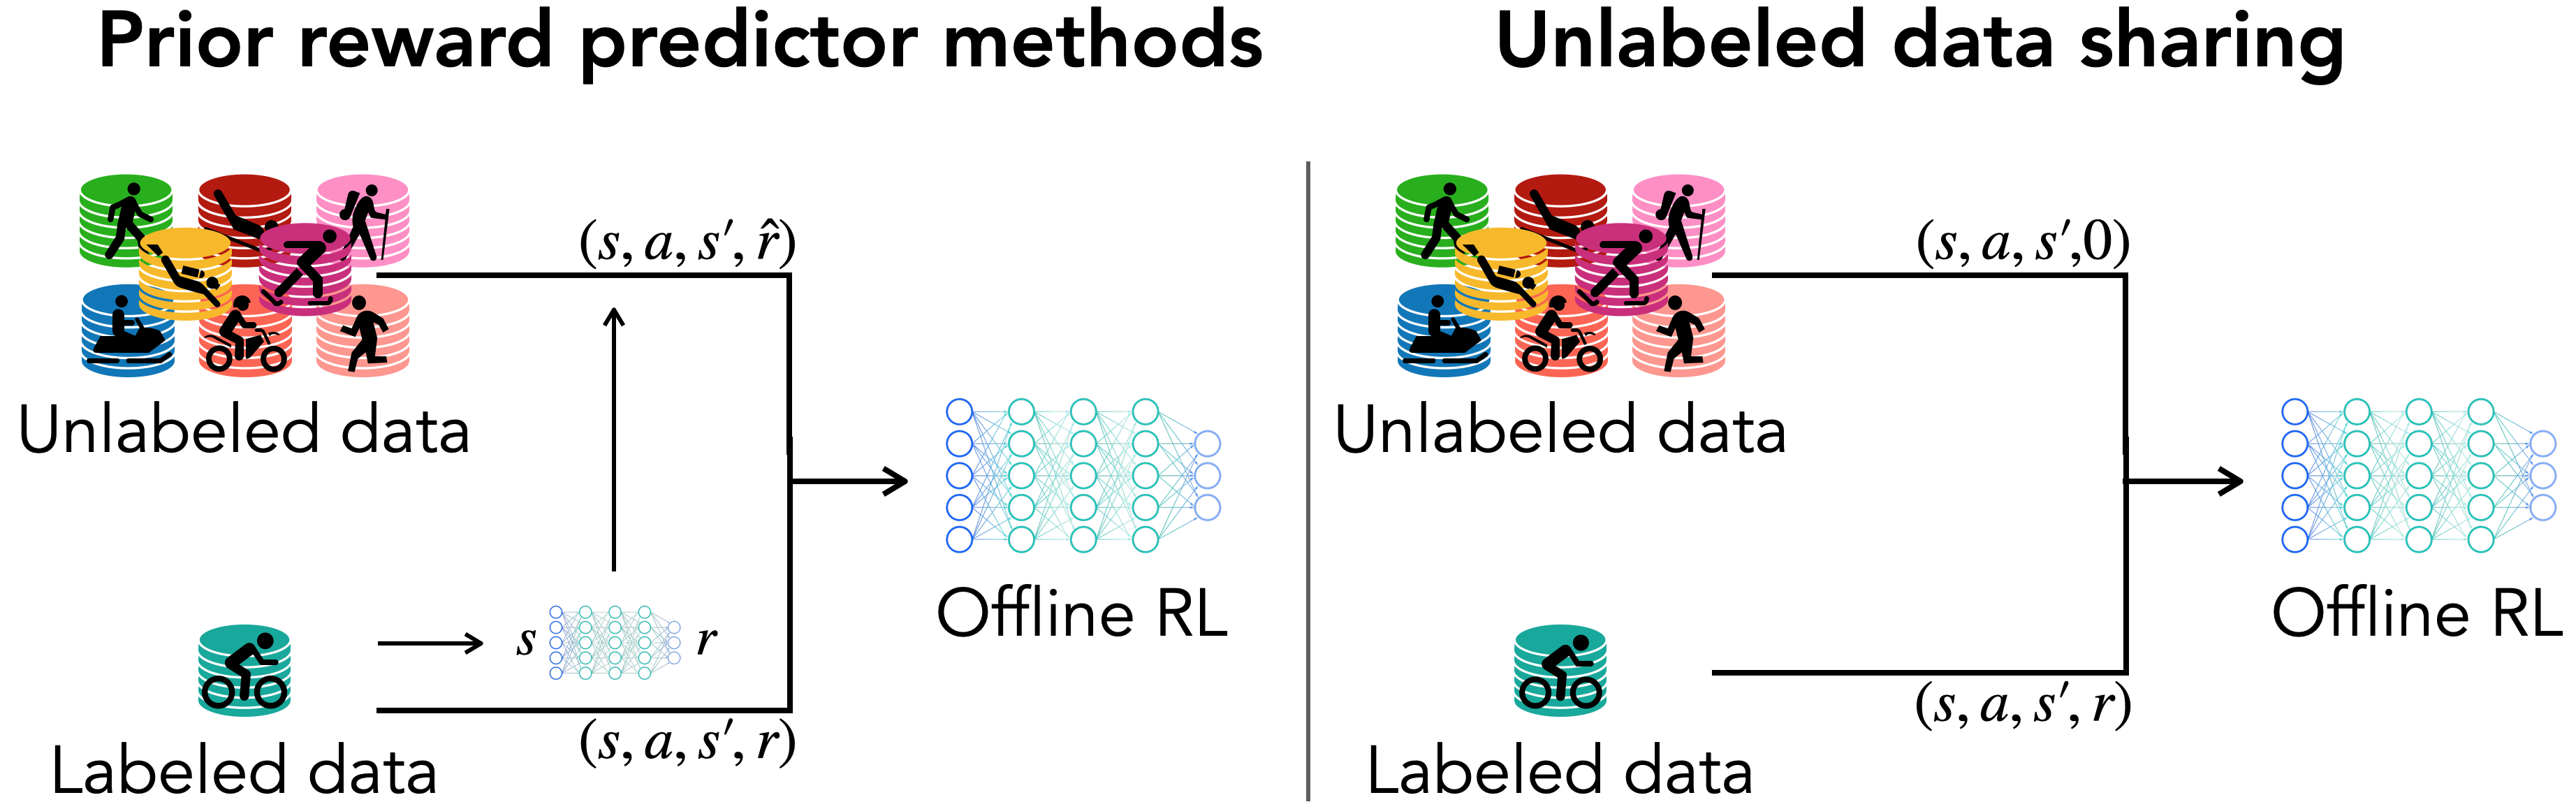
\includegraphics[width=0.48\textwidth]{chapters/uds/teaser_new.png}
    \vspace{-0.2cm}
    \caption{\footnotesize  Overview of various methods dealing with unlabeled offline data. UDS is a simple method compared to the complex reward learning approaches yet achieves effective results.}
    \vspace{-0.4cm}
    \label{fig:uds_teaser}
\end{figure}

% In this paper, we make the potentially surprising observation that prior data such as data from other tasks can be utilized with na\"{i}ve constant reward labels in offline RL, which corresponds to zero reward or whatever is the minimum reward for the task (which we can set to zero via rescaling, without loss of generality). It may at first seem that such an approach would lead to incorrect solutions due to using the wrong reward values. However, we show that this simple reward relabeling strategy, which we refer to as unlabeled data sharing (UDS), can outperform more sophisticated methods that separately learn a reward model and lead to good results in a range of settings. We visualize UDS along with more complex methods in Figure~\ref{fig:uds_teaser}. Na\"{i}ve UDS does not work in all cases, but we further show that carefully reweighting the unlabeled transitions (to modify their distribution) can significantly increase the applicability of this approach and reduce the effects of reward bias, while still preserving many of the benefits. {We analyze this theoretically and show that, in practice, a method based on conservative data sharing~\citep{yu2021conservative}, which reweights unlabeled data to minimize distributional shift (originally designed for use with ground truth reward labels) can be particularly effective in this role.}

% Our main contribution is the finding that simply labeling unlabeled data with a reward of zero for use in offline RL is surprisingly effective in many cases. We perform extensive theoretical and empirical analysis to study conditions under which this simple approach, UDS, would either excel or fail, and we analyze how reweighting the relabeled data (while still using zero reward as the label) can increase the range of settings when UDS is successful. Our empirical evaluation, conducted over various single-task and multi-task offline RL scenarios such as locomotion, robotic manipulation from visual inputs, and ant-maze navigation shows that this simple zero reward strategy leads to improved performance, even compared to methods that use more sophisticated learning and label propagation strategies to infer rewards. This further supports our hypothesis that relabeling unlabeled data with zero reward is an effective approach for utilizing unlabeled prior data in offline RL.
    
    
\subsection{Related Work}
\label{sec:uds_related}

% \textbf{Offline RL.} Offline RL~\citep{ernst2005tree,riedmiller2005neural,LangeGR12,levine2020offline} considers the problem of learning a policy from a static dataset without interacting with the environment, which has shown promises in many practical applications such as robotic control~\citep{kalashnikov2018scalable,Rafailov2020LOMPO}, NLP~\citep{jaques2019way}, 
% and healthcare~\citep{shortreed2011informing, Wang2018SupervisedRL}. 
% The main challenge of offline RL is the distributional shift between the learned policy and the behavior policy~\citep{fujimoto2018off}, which can cause erroneous value backups. To address this issue, prior methods have constrained the learned policy to be close to the behavior policy via policy regularization~\citep{liu2020provably,wu2019behavior,kumar2019stabilizing, zhou2020plas,ghasemipour2021emaq,fujimoto2021minimalist}, conservative value functions~\citep{kumar2020conservative}, 
% and model-based training with conservative penalties~\citep{yu2020mopo,kidambi2020morel,swazinna2020overcoming,lee2021representation,yu2021combo}. Unlike these prior works, we study how unlabeled data can be incorporated into the offline RL framework.

\textbf{RL with unlabeled data.} Prior works tackle the problem of learning from data without reward labels via either directly imitating expert trajectories~\citep{pomerleau1988alvinn,RossB12,GAIL2016Ho}, learning reward functions from expert data using inverse RL~\citep{abbeel2004apprenticeship,ng2000irl,ziebart2008maximum,finn2016guided,AIRLFu2018,konyushkova2020semi}, or learning a reward / value classifier that discriminates successes and failures~\citep{xie2018few,VICEFu2018,singh2019end,eysenbach2021replacing} in standard online RL settings. 
{Unlike these prior works, the goal of our paper is not to propose a sophisticated new algorithm for reward learning,} but rather to study when the simple solution of using zero as the reward label can work well from offline data. {While} \citet{singh2020cog} also considers relabeling prior data with zero reward in the standard, single-task offline RL setting, {the key distinction is that the unlabeled data in \citet{singh2020cog} cannot solve the target task and \emph{actually} gets zero rewards and is thus labeled with the true reward. Unlike \citet{singh2020cog}, we show that UDS can surprisingly also be effective even when the unlabeled data is incorrectly labeled with zero reward, and discuss how it can be improved (Section~\ref{sec:rebalancing}).}
Additionally, we consider both single-task and multi-task offline RL settings.

\textbf{Data sharing.} 
% Sharing data across different tasks has been found to be effective in multi-task~\citep{eysenbach2020rewriting,kalashnikov2021mt,yu2021conservative} and meta-RL~\citep{dorfman2020offline,mitchell2021offline} and it improves performance significantly in multi-task offline RL. 
As discussed in Section~\ref{sec:cds_method}, prior works share data based on learned Q-values~\citep{eysenbach2020rewriting,li2020generalized} (including our CDS approach), domain knowledge~\citep{kalashnikov2021mt}, and other structural quantities such as distance to goals in goal-conditioned settings~\citep{andrychowicz2017hindsight,liu2019competitive,sun2019policy,lin2019reinforcement,chebotar2021actionable}, or the learned distance with robust inference in the offline meta-RL setting~\citep{li2019multi}. However, all of these either require access to the functional form of the reward for relabling or are limited to goal-conditioned settings. In contrast, we attempt to tackle a more general problem where reward labels are not provided for a subset of the data, and find that a simple approach for relabeling data from other tasks with the constant zero (or the minimal possible reward) can work well. 


% \section{Preliminaries}
\vspace{-0.15cm}
\label{sec:prelim}

\textbf{Offline RL.} Standard RL considers a Markov decision process (MDP), $\mdp =(\states, \actions, P, \gamma, R)$, where $\states$ and $\actions$ denote the state and action spaces respectively, $P(\bs' | \bs, \mathbf{a})$ denotes the dynamics, $\gamma \in [0, 1)$ is the discount factor, and $R$ correspond to the reward function. Offline RL tackles the problem of learning a policy $\pi(\mathbf{a}|\bs)$ from a static dataset with $\mathcal{D}$, generated by a behavior policy $\pi_\beta(\mathbf{a}|\bs)$.


\textbf{Data sharing in offline RL.} Data sharing has been considered in the multi-task offline RL setting where there is a static multi-task dataset with $\mathcal{D} = \cup_{i=1}^N \mathcal{D}_i$ where $N$ is the number of tasks. Prior works~\citep{kalashnikov2021mt,eysenbach2020rewriting,yu2021conservative} show that sharing data from different tasks to task $i$ to be conducive. To do so, these prior methods assume access to the functional form of the reward $r_i$. This is a strong assumption in practice, as it necessitates access to a functional (programmatic) form for the reward function. In offline RL, it might be desirable to simply label the reward function by hand, but then the algorithm does not have access to the functional form of the reward, and all unlabeled data also needs to be labeled by hand for use with such methods. Our aim in this paper is to utilize unlabeled data without any reward labels at all.
If however functional access to the reward \emph{is} available, a simple strategy is to na\"ively share data across all tasks, which we refer to as Sharing All. Formally, Sharing All defines the dataset of transitions relabeled from task $j$ to task $i$ as $\mathcal{D}_{j \rightarrow i}$ and the method can be then defined as
    $\mathcal{D}^\mathrm{eff}_i := \mathcal{D}_i \cup ( \cup_{j \neq i} \mathcal{D}_{j \rightarrow i})$,
where $\mathcal{D}^\mathrm{eff}_i$ denotes the effective dataset for task $i$. Therefore, the policy optimization objective in Sharing All can be written as follows:
\begin{equation*}
     \forall i \in [N], ~~\pi^*(\mathbf{a}|\bs, i) := \arg \max_{\pi}~~ J_{\mathcal{D}^\mathrm{eff}_i}(\pi) - \alpha D(\pi, \pi^\mathrm{eff}_\beta),
\end{equation*}
where $\pi_\beta^\mathrm{eff}(\mathbf{a}|\bs, i)$ is the effective behavior policy for task $i$ denoted as $\pi_\beta^\mathrm{eff}(\mathbf{a}|\bs, i) := |\mathcal{D}^\mathrm{eff}_i(\bs, \mathbf{a})| / |\mathcal{D}^\mathrm{eff}_i(\bs)|$, $J_{\mathcal{D}^\mathrm{eff}_i}(\pi)$ denotes the average return of policy $\pi$ in the empirical MDP induced by the effective dataset, and $D(\pi, \pi^\mathrm{eff}_\beta)$ denotes a divergence measure (e.g., KL-divergence~\citep{jaques2019way,wu2019behavior}, fisher divergence~\citep{kostrikov2021offline}, MMD distance~\citep{kumar2019stabilizing} or $D_{\text{CQL}}$ from conservative Q-values~\citep{kumar2020conservative}) between the learned policy $\pi$ and the effective behavior policy $\pi_\beta^\mathrm{eff}$. Note that conservative Q-values refer to the Q-value for a given policy corresponding to a modified reward function $r(\bs, \mathbf{a}) - \alpha \pi(\mathbf{a}|\bs) \cdot (\pi(\mathbf{a}|\bs) / \pi_\beta(\mathbf{a}|\bs) - 1)$, computed on the empirical MDP. We also note that Sharing All can be easily adapted to the single-task setting where there is only one target task with labeled data $\mathcal{D}_\text{L}$ and unlabeled prior data $\mathcal{D}_\text{U}$. While data sharing tends to show promising results, it requires the assumption of the access to the functional form of the reward function. We instead focus on the data sharing problem where we do not make such an assumption and instead, only have the reward labels for originally commanded task, which we will discuss in the following section.




\section{How To Use Unlabeled Data in Offline RL}
\vspace{-0.1cm}
\label{sec:method}
Arguably the easiest approach to utilize unlabeled data in offline RL is to simply assign the lowest possible reward to all the transitions in the unlabeled data, which we will assume to be $0$ without loss of generality, and use this data for training the underlying offline RL method. We will refer to this approach as UDS. We will show that, although this strategy might seem simplistic, in fact, it can work well both in theory and practice, when the dataset composition and the task satisfies certain criteria. Not all tasks and datasets satisfy these criteria, but we will argue that many realistic offline RL problems do satisfy them. For example, UDS can work well in a problem where the labeled data consists of high-quality, near-expert demonstrations, while the unlabeled data consists of mediocre or low-reward interactions in the environment, as is often the case in robotics~\citep{xie2019improvisation}. 
We will analyze the performance of this approach theoretically in Section~\ref{sec:uds_theory} and empirically in Section \ref{sec:empirical_analysis}.

Although the simple UDS approach can perform well in some scenarios, relabeling with zero reward of course also biases the learning process. We therefore further show that reward bias can be mitigated if the unlabeled transitions are additionally reweighted, so as to change the unlabeled data distribution (while still using a label of zero for all unlabeled data). While such reweighting reduces the sample size, it can provide an overall benefit by reducing the reward bias \ak{and distributional shift}. We will derive the optimal scheme for reweighting the transitions in the unlabeled dataset that minimizes the impact of reward bias in Section~\ref{sec:rebalancing}. Surprisingly, our analysis reveals that a near-optimal solution to reducing reward bias is to combine \uds\ with an already existing reweighting scheme for multi-task offline RL with full reward information. For example, one can choose to reweight unlabeled data with the  {CDS} scheme of \citet{yu2021conservative}, which preferentially upweights transitions based on their conservative Q-values.

\vspace{-0.1cm}
\subsection{Theoretical Analysis of UDS in Offline RL}
\vspace{-0.1cm}
\label{sec:uds_theory}
In this section, we will derive a performance bounds for \uds\ that allow us to understand several cases when this simple baseline approach still works well. We will show that the increase in the effective dataset size can often outweigh the bias incurred from using the wrong reward in several practical situations. We will also discuss conditions on the data composition and the relative distributions of labeled and unlabeled data that enable UDS to be successful.
Formally, UDS trains on an effective dataset given by:
\begin{equation}
    \mathcal{D}^\mathrm{eff} = \mathcal{D}_\mathrm{L} \cup \{(\bs_j, \mathbf{a}_j, \bs'_j, 0) \in \mathcal{D}_{\mathrm{U}}\}. \label{eq:uds}
\end{equation}
We now present a policy improvement guarantee for UDS below, and then analyze the bound under special conditions. Our theoretical result builds on techniques for showing safe policy improvement bounds~\citep{laroche2019safe,kumar2020conservative,yu2021conservative}. 

\begin{table*}[t]
\vspace{-0.15cm}
\caption{\footnotesize Summary of scenarios where UDS is expected to work and where it is not expected to work. \textbf{L} denotes the characteristics of labeled data, \textbf{U} denotes characteristics of unlabeled data. Limited/Abundant refers to the relative amount of data available
High-quality/medium-quality/low-quality refers to the actual performance of the behavior policy generating the datasets. Narrow/broad refers to the relative state coverage of the datasets that we study where high coverage can lead to low distributional shift during offline RL. We provide intuitions on why UDS works or does not work under each scenario and refer to the cases shown in our analysis in Section~\ref{sec:uds_theory}.}
\vspace{-0.43cm}
\begin{center}
\scriptsize
\resizebox{\textwidth}{!}{\begin{tabular}{l|r|l}
\toprule
 \textbf{Scenarios} & \textbf{UDS} & \textbf{Intuition} \\
 \midrule
  \textbf{L}: limited + high-quality + narrow, \textbf{U}: abundant + low/medium-quality + broad & \textcolor{green}{\checkmark} & increase coverage (case \textbf{\rom{2}} and \textbf{\rom{3}})\\
  \textbf{L}: limited + medium-quality + narrow, \textbf{U}: \ak{abundant} + low/medium-quality + broad &  \textcolor{red}{$\times$} & reward bias outweighs high coverage\\
  \textbf{L}: limited + high-quality + narrow, \textbf{U}: abundant + high-quality + narrow &   \textcolor{green}{\checkmark} & identical distribution (case \textbf{\rom{1}})\\
  \textbf{L}: limited + low-quality + narrow, \textbf{U}: abundant + high-quality + narrow & \textcolor{green}{\checkmark} & increase data quality (case \textbf{\rom{2}})\\
\bottomrule
\end{tabular}}
\end{center}
\vspace{-0.7cm}
\label{tbl:summary_criteria}
\normalsize
\end{table*}

\begin{theorem}[\textbf{Policy improvement guarantee for UDS}] 
\label{prop:uds_ours}
Let $\pi^*_\text{UDS}$ denote the policy learned by UDS, and let $\pi^\mathrm{eff}_\beta(\mathbf{a}|\bs)$ denote the behavior policy for the combined dataset $\mathcal{D}^\mathrm{eff}$. Then with high probability $\geq 1 - \delta$, $\pi^*_\text{UDS}$ is a safe policy improvement over $\pi_\beta^\mathrm{eff}$, i.e.,
\begin{align*}
& J(\pi^*_\text{UDS}) \geq J(\pi_\beta^\mathrm{eff}) - \zeta_\text{err} +  \underbrace{\frac{\alpha}{1 - \gamma} D(\pi^*_\text{UDS}, \pi^\mathrm{eff}_\beta)}_{\text{(c): policy improvement}},\\
 & \zeta_\text{err} = \underbrace{\mathrm{RewardBias}(\pi^*_\text{UDS}, \pi^\mathrm{eff}_\beta)}_{ \text{(a)}} \\
 &+\underbrace{\mathcal{O}\left(\frac{\gamma}{(1 - \gamma)^2}\right) \mathbb{E}_{\bs, \mathbf{a} \sim \widehat{d}^{\pi}}\left[\sqrt{\frac{D_{\text{CQL}}(\pi^*_\text{UDS}, \pi^\mathrm{eff}_\beta)(\bs)}{|\mathcal{D}^\mathrm{eff}(\bs)|}} \right]}_{\text{(b): sampling error}},\\
\!\!\!\!\!\!\!\!\!\!\!\!\!\!\!\!\!\!\!\!\!\!\!(a) &:= \frac{\sum_{\bs, \mathbf{a}}\Delta\left(\widehat{d}^{\behavior^\mathrm{eff}}, \widehat{d}^{\pi^*_\text{UDS}}\right)  \cdot (1 - f(\bs, \mathbf{a})) \cdot r(\bs, \mathbf{a})}{1 - \gamma},
\end{align*}
where we use the notation $f(\bs, \mathbf{a}) := \frac{|\mathcal{D}_\mathrm{L}(\bs, \mathbf{a})|}{|\mathcal{D}^\mathrm{eff} (\bs, \mathbf{a})|}$ and $\Delta(\widehat{d}^{\behavior^\mathrm{eff}}, \widehat{d}^{\pi^*_\text{UDS}}) = \widehat{d}^{\behavior^\mathrm{eff}}(\bs, \mathbf{a}) - \widehat{d}^{\pi^*_\text{UDS}}(\bs, \mathbf{a})$. 
\end{theorem}
A proof for Theorem~\ref{prop:uds_ours} is provided in Appendix~\ref{proof:uds_proof}. Intuitively, term (a) corresponds to the potential suboptimality incurred as a result of using the wrong reward, term (b) corresponds to the suboptimality induced due to sampling error. Finally, term (c) corresponds to the policy improvement in the empirical MDP induced by the transitions in $\mathcal{D}^\mathrm{eff}$ that occurs as a result of offline RL. Intuitively, we expect that including more unlabeled data will reduce the sampling error (b) and potentially increase how much we can improve the policy (c), while potentially increasing the reward bias term (a). The key question is under which conditions we would expect the increase in bias (a) to be lower than the decrease in term (b) obtained from using the unlabeled data. We examine this question below, presenting a few common cases where we expect this tradeoff to be favorable.

\textbf{(\rom{1}) Unlabeled data is distributed identically as labeled data.} The first special case we consider is when the distribution of state-action pairs in $\mathcal{D}_\mathrm{L}$ is {identical} to the distribution of state-action pairs in the unlabeled dataset $\mathcal{D}_U$. This can arise in many application domains, such as in robotics~\citep{xie2019improvisation,dasari2020robonet}, where a large amount of offline data is available, but only a limited uniformly-selected fraction of it can be annotated with rewards. In this case, the fraction $f(\bs, \mathbf{a})$ takes on identical values for all state-action pairs, and term (a) simply reverts to be a difference between the performance of the effective behavior policy and the learned policy, in the empirical MDP. Since offline RL algorithms would improve over the effective behavior policy in the empirical MDP, this term is negative and hence, no additional suboptimality is incurred in the reward bias term. Moreover, the sampling error term \final{(b)} reduces when more data is utilized. Thus, in this case, \uds\ improves performance due to an increase in the dataset size $|\mathcal{D}^\mathrm{eff}(\bs)|$, without incurring a cost due to the wrong reward.   

\textbf{(\rom{2}) Quality of the unlabeled dataset.} In practice, we are often provided with a small amount of high-quality reward annotated demonstration data, and a lot of unlabeled prior data of low or mediocre quality. In this case, assigning a low reward to the transitions in the unlabeled dataset does not negatively affect policy performance significantly because the bias due to wrong reward is low (due to low-quality of labeled data) and reduces sampling error (term \final{(b)}). On the other hand, when the unlabeled data is of high quality and large in size compared to the labeled dataset, even then the performance of the policy $J(\pi^*_{\mathrm{UDS}})$ can be improved by using this unlabeled set since \uds\ improves $J(\pi_\beta^\mathrm{eff})$. 

\textbf{(\rom{3}) Large unlabeled datasets for long-horizon tasks.} Another scenario when \uds\ relabeling will be beneficial to do compared to not using the unlabeled data at all is in long-horizon tasks (large value of $1/(1 - \gamma)$), where a lot of unlabeled data is available, while the labeled dataset, $\mathcal{D}_\mathrm{U}$ is relatively very small. Define  $H = \frac{1}{1 - \gamma}$; then in the case that $|\mathcal{D}^\mathrm{eff}(\bs)| = \Omega(H^2) |\mathcal{D}_\mathrm{L}(\bs)|$, the sampling error term (term \final{(b)}) will consist of one less factor of $1/(1 - \gamma)$ when utilizing unlabeled data, compared to when it is not. Since the sampling error grows quadratically in the horizon, whereas the reward bias only grow linearly, a reduction in this term by increasing $|\mathcal{D}^\mathrm{eff}(\bs)|$ (i.e., denominator) can improve compared to only using the labeled data, $\mathcal{D}_\mathrm{L}$. Thus, even though the rewards may be biased, the addition of large amounts of unlabeled, diverse data in long-horizon tasks can help despite the reward bias incurred. 

We empirically verify that \uds\ indeed helps in the special cases discussed above in Section~\ref{sec:empirical_analysis}. However, there are also cases where \uds\ does not help because of large suboptimality induced due to term (a). In Table \ref{tbl:summary_criteria}, we present a summary of the scenarios under which we expect \uds\ will help or hurt performance.
As an example of the latter, when the amount of unlabeled data, $\mathcal{D}_\mathrm{U}$ is not very large compared to the labeled dataset, such that a decrease in sampling error does not outweigh the suboptimality induced by reward bias, we should not expect \uds\ to attain very good performance, which we empirically show in Appendix~\ref{app:unlabeled_dataset_size_analysis}. To handle such cases, our key idea is to re-weight the unlabeled dataset before using it for offline RL training reduce the sampling error and reward bias.

\vspace{-0.05cm}
\subsection{Reducing Reward Bias by Reweighting Data}
\label{sec:rebalancing}
\vspace{-0.05cm}
As discussed above, one way to reduce the suboptimality induced due to reward bias is by preferentially reweighting transitions in the unlabeled data. We would hope that such a scheme can provide a favorable bias-sampling error tradeoff, even though it reduces sample size. In this section, we will derive an optimized reweighting scheme that attains a favorable tradeoff. \ak{Intuitively, this optimized scheme suggests that reweighting must reduce distributional shift against the state-action marginal of the policy obtained by running offline RL on only the transitions in the labeled data.}
This scheme intuitively matches the conservative data sharing method~\citet{yu2021conservative} previously proposed for (fully-labeled) multi-task offline RL. We will show that this conservative sharing approach reduces reward bias, controls distributional shift that appears in the numerator of sampling error, and increases the sample size.   

Formally, we will derive this reweighting scheme from the perspective of optimizing the effective behavior policy, $\pi^\mathrm{eff}_\beta$ induced by the dataset $\mathcal{D}$ after preferentially sharing transitions from the unlabeled data, so as to minimize reward bias and sampling error, while improving the dataset quality. For understanding purposes, we begin by deriving the choice of $\pi^\mathrm{eff}_\beta$ that reduces only the reward bias component:
\begin{theorem}[\textbf{Optimized reward bias reduction}] 
\label{prop:reward_bias_theorem}
The optimal effective behavior policy that minimizes the bias (a) in Theorem~\ref{prop:uds_ours}, $\mathrm{RewardBias}(\pi, \pi^\mathrm{eff}_\beta)$, satisfies
\begin{align*}
    \widehat{d}^{\widehat{\pi}^\mathrm{eff}_\beta}(\bs, \mathbf{a}) \propto  \sqrt{{d}_\mathrm{L}(\bs, \mathbf{a}) d^{\pi}(\bs, \mathbf{a})},
\end{align*}
where $d^{\pi}$ denotes the state-action marginal of a policy $\pi$, and $d_\mathrm{L}(\bs, \mathbf{a})$ denotes the density of state-action pair $(\bs, \mathbf{a})$ under the labeled dataset.
\end{theorem}
A proof of Theorem~\ref{prop:reward_bias_theorem} is provided in Appendix~\ref{sec:small_reward_bias}. The expression implies that the state-action marginal of the effective behavior policy (i.e., the rebalanced dataset distribution) must place mass on state-action tuples that are both likely to under the learned policy $d^{\pi}$ and appear frequently in the distribution induced by the labeled dataset $\widehat{d}_\mathrm{L}$. However, note that Theorem~\ref{prop:reward_bias_theorem} only accounts for the reward bias and not the other terms pertaining to sampling error and the performance of the effective behavior policy that appear in Theorem~\ref{prop:uds_ours}. To address both of these issues, in our next theoretical result, Theorem~\ref{thm:with_all_sources}, we derive the reweighting distribution that controls all the terms.
\begin{theorem}[\textbf{Optimized reweighting unlabeled data}; Informal]
\label{thm:with_all_sources}
The optimal effective behavior policy that maximizes a lower bound on $J(\pi_\beta^\mathrm{eff}) - \left[(a) + (b)\right]$ in Theorem~\ref{prop:uds_ours} satisfies $d^{\widehat{\pi}_\beta^\mathrm{eff}}(\bs, \mathbf{a}) = p^*(\bs, \mathbf{a})$, where:
\begin{align*}
    p^* = \arg\min_{p \in \Delta^{|\mathcal{S}||\mathcal{A}|}}&~ \sum_{\bs, \mathbf{a}} C_1 \frac{\widehat{d}^\pi(\bs, \mathbf{a})}{\sqrt{p(\bs, \mathbf{a})}} + C_2 |\widehat{d}_\mathrm{L}(\bs, \mathbf{a})| \frac{\widehat{d}^\pi(\bs, \mathbf{a})}{p(\bs, \mathbf{a})}, 
\end{align*}
where $C_1$ and $C_2$ are universal positive constants that depend on the sizes of the labeled and unlabeled datasets.
\end{theorem}
A proof of Theorem~\ref{thm:with_all_sources} along with a more formal statement listing the constants $C_1$ and $C_2$ is provided in in {Appendix~\ref{proof:all_sources}}. The first term in the optimization objective of $p^*$ appearing above arises from the sampling error term, while the second term corresponds to the reward bias term in Theorem~\ref{prop:uds_ours}. The optimal solution for $p^*$ must place high density on $(\bs, \mathbf{a})$ pairs where $\widehat{d}^\pi(\bs, \mathbf{a})$ is high, because this would reduce the objective in the optimization problem above. This corroborates the analysis of \citet{yu2021conservative}, which shows that utilizing a reweighting scheme that reduces distributional shift (i.e., makes $\pi(\mathbf{a}|\bs)/\widehat{\pi}^\mathrm{eff}_\beta(\mathbf{a}|\bs)$ or \ak{equivalently}, as we find, making $\widehat{d}^\pi(\bs, \mathbf{a})/\widehat{d}^{\pi_\beta^\mathrm{eff}}(\bs, \mathbf{a})$ smaller) will control sampling error, and give rise to performance benefits. In addition, as also shown in Theorem~\ref{prop:reward_bias_theorem}, the reward bias term is also controlled when low distributional shift appears. This means that rebalancing the dataset to control distributional shift between the learned policy $\widehat{d}^\pi(\bs, \mathbf{a})$ and $\widehat{d}^{\pi^\mathrm{eff}_\beta}(\bs, \mathbf{a})$ is effective in unlabeled settings as well.


\begin{table*}[t]
\vspace{-0.2cm}
\caption{\footnotesize Results on single-task environments {hopper} and {AntMaze} from the D4RL~\citep{fu2020d4rl} benchmark. The numbers are averaged over three random seeds. We only bold the best-performing method that does not have access to the true reward for relabeling. UDS outperforms No Sharing in three out of the four settings while achieving competitive performances compared to Sharing All in all the settings. CDS+UDS further improves over UDS in three out of four settings.}
\vspace{-0.24cm}
\begin{center}
\resizebox{\textwidth}{!}{\begin{tabular}{l|l|l|rrrrrr|rr}
\toprule
& & & & & & & & & \multicolumn{2}{c}{\textbf{Oracle Methods}} \\
 \textbf{Environment} & \textbf{Labeled data} & \textbf{Unlabeled data}   & \textbf{CDS+UDS}   & \textbf{UDS}         & \textbf{No Sharing} & \textbf{Reward Pred.} & \textbf{VICE} & \textbf{RCE}  & \textbf{CDS} & \textbf{Sharing All} \\
 \midrule
 D4RL hopper & expert & random & \textbf{81.5}  & 78.6 & 77.1 & 67.6 & n/a & n/a & 83.3 & 86.1\\
  & expert & medium & \textbf{78.3}  & 64.4 & 77.1 & 51.7 & n/a & n/a & 82.5 & 64.6\\
\midrule
D4RL AntMaze & expert & medium-play & 82.6  & \textbf{82.7} & 17.2 & 0.0 & 0.0 & 0.0 & 83.5 & 83.1 \\
 & expert & large-play & \textbf{47.1} & 33.1 & 0.7 & 0.0 & 0.0 & 0.0 & 46.1 & 50.2\\
\bottomrule
\end{tabular}}
\end{center}
\vspace{-0.7cm}
\label{tbl:single_task}
\normalsize
\end{table*}

While the scheme derived above can, in principle, be implemented exactly in practice, it would require computing state-marginals. Since, computing state marginals accurately in an offline setting has been an outstanding challenge,
we instead can utilize a reweighting scheme that corrects for distributional shift approximately without needing state-marginals. One of such methods is conservative data sharing (CDS)~\citep{yu2021conservative} that can be implemented without requiring additional components beyond the machinery of the offline RL method. Formally, CDS is given by:
\begin{equation*}
    \mathcal{D}^\mathrm{eff}_i = \mathcal{D}_i \cup ( \cup_{j \neq i}\{(\bs_j, \mathbf{a}_j, \bs'_j, r_i) \in \mathcal{D}_{j \rightarrow i}: \Delta^\pi(\bs, \mathbf{a}) \geq 0\}),
\end{equation*}
where $\bs_j, \mathbf{a}_j, \bs'_j$ denote the transition from $\mathcal{D}_j$, $r_i$ denotes the reward of $\bs_j, \mathbf{a}_j, \bs'_j$ relabeled for task $i$, $\pi$ denotes the task-conditioned policy $\pi(\cdot|\cdot, i)$, $\Delta^\pi(\bs_j, \mathbf{a}_j)$ is the condition that shares data only if the expected conservative Q-value of the relabeled transition exceeds the top $k$-percentile of the conservative Q-values of the original data. In our experiments and analysis in Section \ref{sec:exp}, we find that utilizing CDS improves performance over simply training with \uds\ in a number of domains supporting the theoretical analysis. 


\subsection{Why Can We Expect UDS to Outperform Reward Prediction Methods?}
\label{sec:reward_predictor_discussion}
While we have discussed various conditions where we would expect UDS (with or without various reweighting methods) to improve final performance over an approach that does not utilize the unlabeled data, it is also instructive to consider how it comes to a method that instead trains an approximate reward function, $\widehat{r}_\phi(\bs, \mathbf{a})$ using the labeled data, and then uses this approximate reward to annotate the unlabeled data. In our experiments, we will show, perhaps surprisingly that UDS often outperforms prior reward learning methods. In this section, we provide some intuition for why. 
First, we note the following generic expression for reward bias (term (a) in Theorem~\ref{prop:uds_ours}) for any approach:
\begin{align*}
    \mathrm{RewardBias}(\pi, \pi^\mathrm{eff}_\beta) = \frac{\sum_{\bs, \mathbf{a}} \Delta\left(\widehat{d}^{\behavior^\mathrm{eff}}, \widehat{d}^{\pi}\right) \cdot \Delta r(\bs, \mathbf{a})}{1 - \gamma},
\end{align*}
where $\Delta r(\bs, \mathbf{a})$ is the error in the reward applied to the unlabeled data, such that $\Delta r(\bs, \mathbf{a}) = (1 - f(\bs, \mathbf{a})) r(\bs, \mathbf{a})$ for UDS, and $\Delta r(\bs, \mathbf{a}) = r(\bs, \mathbf{a}) - \widehat{r}_\phi(\bs, \mathbf{a})$ for a reward prediction method. Note that while for UDS, $\forall~\bs, \mathbf{a}, ~\Delta r(\bs, \mathbf{a}) \geq 0$, this is not necessarily the case for a generic reward prediction method.

\textbf{UDS.} Since $\Delta r(\bs, \mathbf{a}) \geq 0$ for all state-action tuples, state-action pairs that appear more frequently under the learned policy compared to the effective behavior policy, i.e., when $\Delta\left(\widehat{d}^{\behavior^\mathrm{eff}}, \widehat{d}^{\pi}\right) < 0$, contribute to reducing the suboptimality induced due to reward bias. 

\textbf{Reward prediction.} When $\Delta r(\bs, \mathbf{a}) = r(\bs, \mathbf{a}) - \widehat{r}_\phi(\bs, \mathbf{a})$, $\Delta r(\bs, \mathbf{a})$ may not be positive on all state-action tuples, and thus reward prediction methods fail to reduce the contribution of such state-action pairs in term (a). Since policy optimization will seek out those policies that maximize $\widehat{d}^\pi(\bs, \mathbf{a})$ on state-action pairs with high rewards, state-action pairs where $\Delta(\widehat{d}^{\pi_\beta^\mathrm{eff}}, \widehat{d}^\pi) < 0$ (i.e., state-action pairs that appear more under the learned policy) are likely to also have $\Delta r(\bs, \mathbf{a}) < 0$. This ``exploitation'' inhibits the correction of reward bias and provides an explanation for why reward prediction approaches may still not perform well due to overestimation errors in the reward function.  


\newcommand{\CC}{\cellcolor{Gray}}
\definecolor{Gray}{gray}{0.9}

\vspace{-0.2cm}
\subsection{Experimental Evaluation of UDS and CDS+UDS}
\label{sec:uds_exp}
\vspace{-0.2cm}
In our experiments, we aim to evaluate whether the theoretical potential for simple minimum-reward relabeling to attain good results is reflected in benchmark tasks and more complex offline RL settings. In particular, we will study: \textbf{(1)} can UDS match or exceed the performance of sophisticated reward inference methods and methods with oracle reward functions in simulated locomotion and navigation tasks? \textbf{(2)} can combining with CDS further improve the results achieved by UDS?, \textbf{(3)} how does UDS behave with and without combining with an optimized reweighting strategy in multi-task offline RL settings?, \textbf{(4)} under which conditions does UDS work and not work and does optimizing for reweighting via CDS help?


\textbf{Comparisons.} 
We evaluate multiple approaches alongside with \textbf{UDS} and \textbf{CDS+UDS}:
\textbf{No Sharing}, which uses the labeled data only without using any of the unlabeled data, \textbf{Reward Predictor}, which is trained via supervised classification or regression to directly predict the reward in sparse and dense reward settings respectively, \textbf{VICE}~\citep{fu2018variational} and \textbf{RCE}~\citep{eysenbach2021replacing}, inverse RL methods only applicable to sparse reward settings, that learn either a reward or Q-function classifier from both the labeled data and unlabeled data (treated as negatives) and then annotate the unlabeled data with the learned classifier, 
In the multi-task setting, we modify \textbf{VICE} and \textbf{RCE} accordingly by extracting transitions with reward labels equal to 1 and treating these datapoints as positives to learn the classifier for each task. We also train \textbf{No Sharing}, \textbf{Reward Predictor}, \textbf{VICE} and \textbf{RCE}, but adapt them to the offline setting using CQL, i.e. the same underlying offline RL method as in \textbf{UDS} and \textbf{CDS+UDS}.
For more details on experimental set-up and hyperparameter settings, please see Appendix~\ref{app:uds_details}. 
\rebuttal{We also include evaluations of our methods under different quality of the relabeled data in Appendix~\ref{app:data_quality} and comparisons to model-based offline RL approaches in Appendix~\ref{app:mbrl} and prior methods~\citep{yang2021representation,yang2021trail} that leverage unlabeled data for representation learning instead of sharing directly in Appendix~\ref{app:pretrained_reps}.}

\textbf{Datasets and tasks.} To answer questions (1) and (2), we perform empirical evaluations on two state-based single-task locomotion datasets. To answer question (3), we further evaluate all methods on three state-based multi-task datasets that consist of robotic manipulation, navigation and locomotion domains respectively and one image-based multi-task manipulation dataset from Section~\ref{sec:cds_exp}.

% \begin{figure}[ht]
%     \centering
%     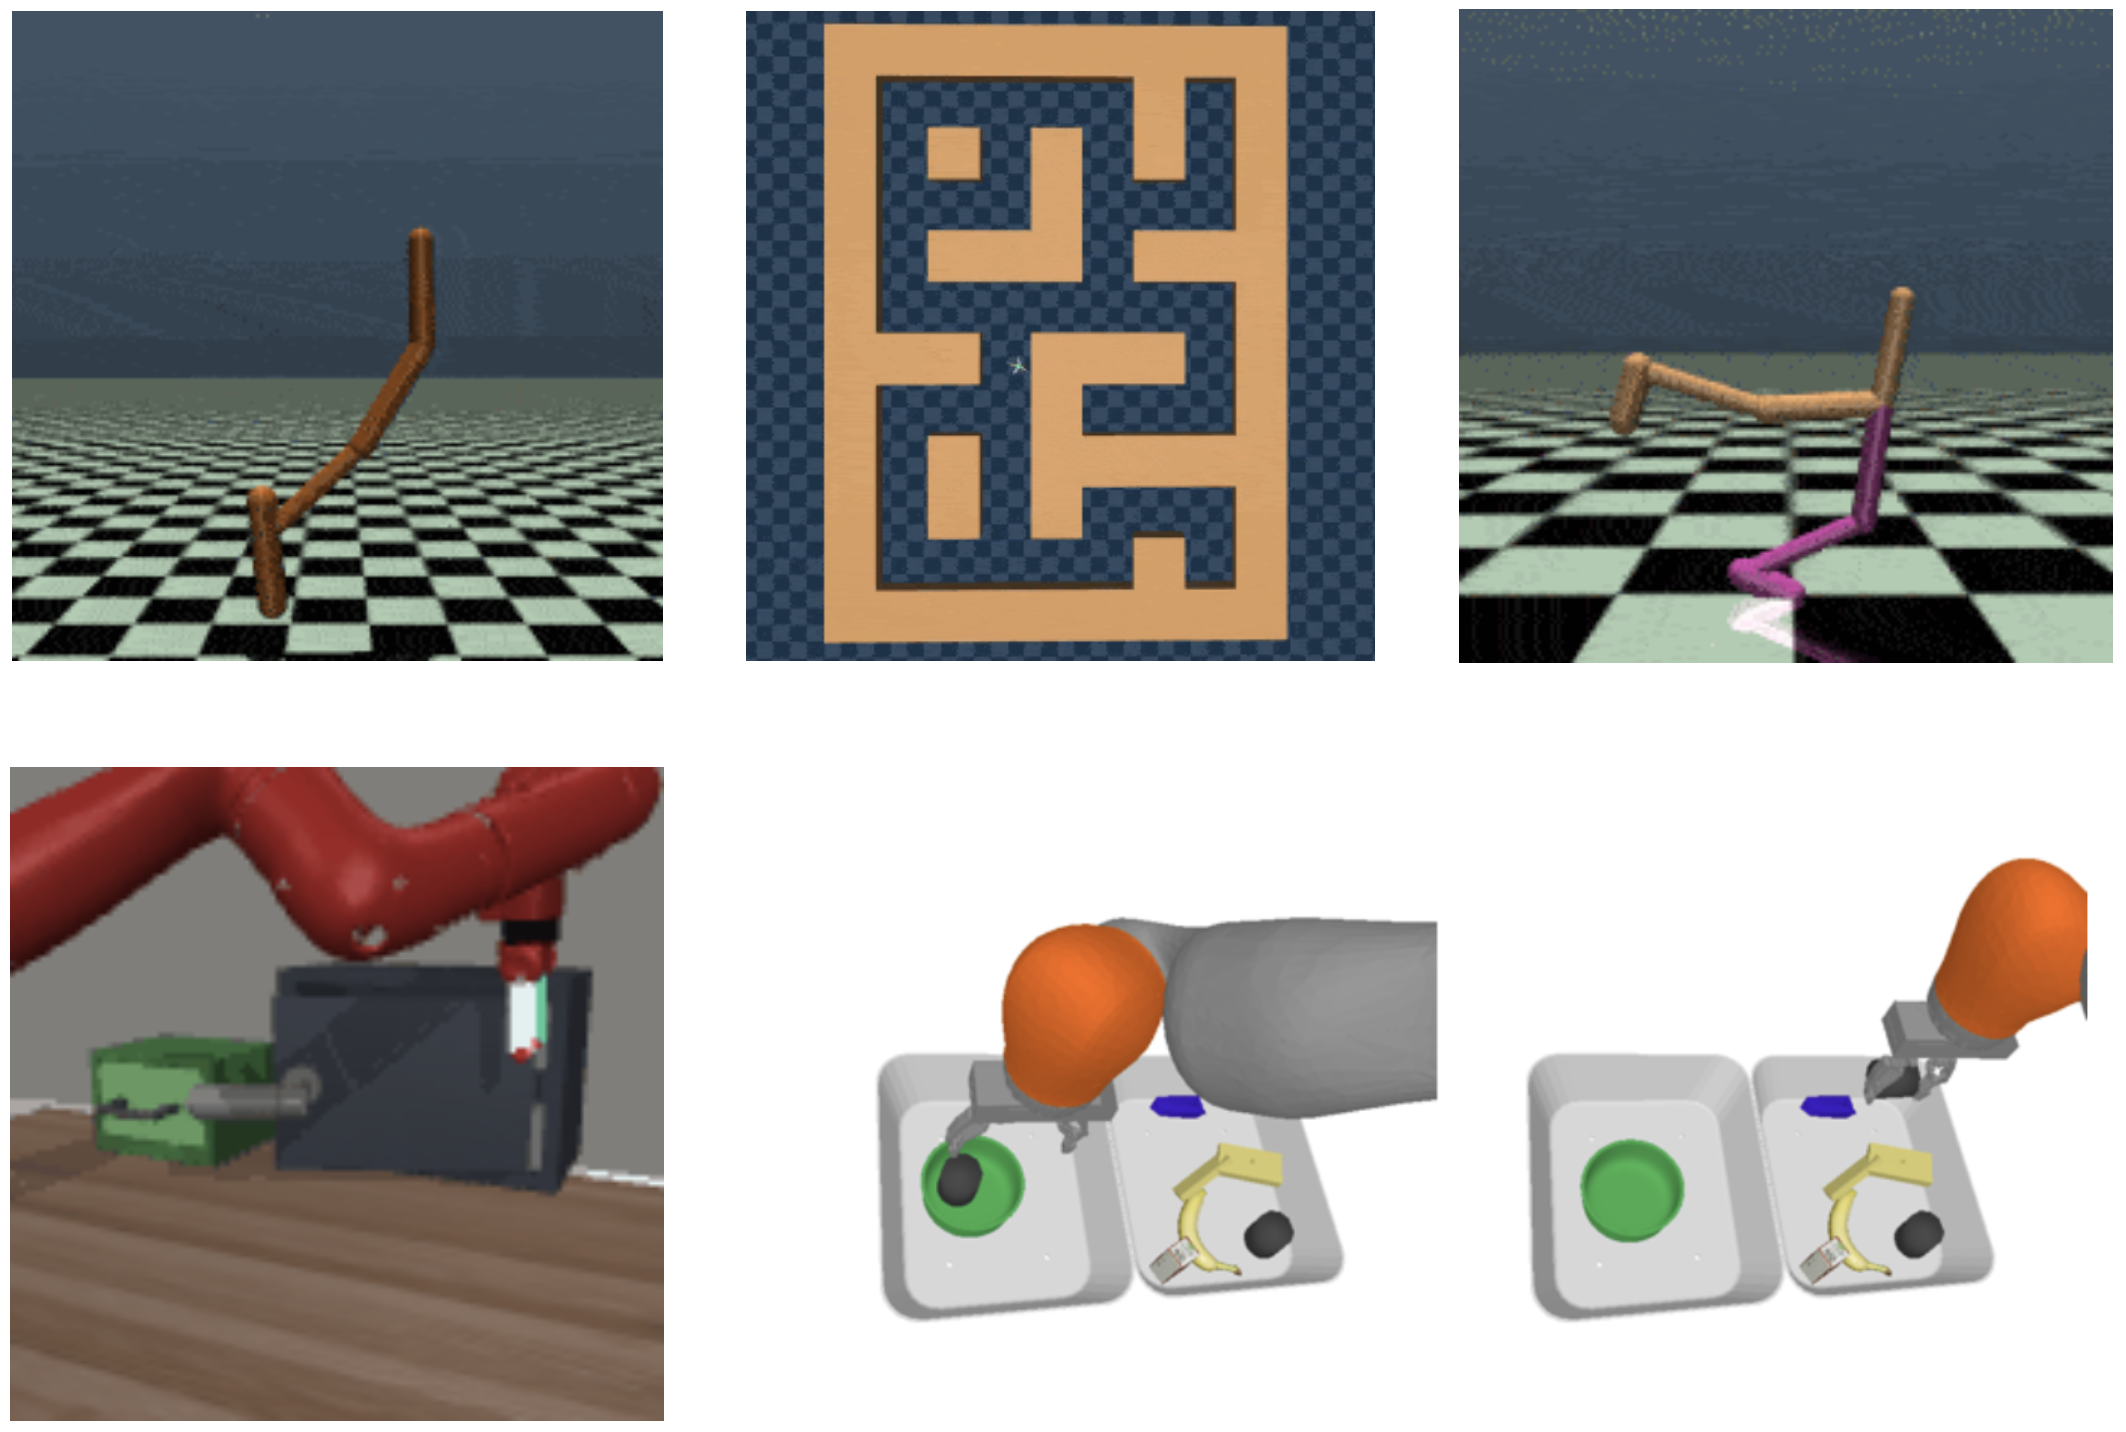
\includegraphics[width=0.35\textwidth]{chapters/uds/env.png}
%     \vspace{-0.33cm}
%     \caption{\footnotesize  Environments (from left to right):  single-task hopper, single-task and multi-task AntMaze, multi-task walker, multi-task Meta-World, and multi-task vision-based pick-place tasks.}
%     \vspace{-0.35cm}
%     \label{fig:env}
% \end{figure}

\noindent \textbf{Single-task domains \& datasets.} We adopt two environments: hopper and the AntMaze from the D4RL benchmark~\citep{fu2020d4rl} for evaluation in the single-task setting. For the hopper environment, we consider two scenarios where we have 10k labeled data from the {hopper-expert} and 1M unlabeled transitions from the {hopper-random} datasets and {hopper-medium} datasets respectively. This setup is resembles practical problems where unlabeled data is of low-quality and even, irrelevant to the target task. For AntMaze, following the setup in \cite{yang2021trail}, we use 10k expert transitions as the labeled data and the entire datasets of {large-play} and {medium-play} as the unlabeled data.


\begin{table*}[ht]
\vspace{-0.2cm}
\caption{\footnotesize We perform an empirical analysis on the single-task environment \texttt{hopper} from D4RL~\citep{fu2020d4rl} benchmark to test the sensitivity of UDS under the data quality and data coverage for both the labeled task data and unlabeled data. The numbers are averaged over \final{ten} random seeds. We bold the best method without true reward relabeling. UDS outperforms No Sharing in 5 out of 6 settings while achieving competitive performances compared to Sharing All in 5 out of 6 settings.
CDS+UDS is able to further improve over UDS significantly in such a setting and also outperforms UDS in 5 out of 6 settings in general.
}
\vspace{-0.2cm}
\begin{center}
\resizebox{\textwidth}{!}{\begin{tabular}{l|l|l|rrr|rr}
\toprule
& & & & & & \multicolumn{2}{c}{\textbf{Oracle Methods}} \\
 \textbf{Environment} & \textbf{Labeled data type / size} & \textbf{Unlabeled data type / size}   & \textbf{CDS+UDS}   & \textbf{UDS}         & \textbf{No Sharing} & \textbf{CDS} & \textbf{Sharing All} \\
 \midrule
& \textbf{(a)} expert / 10k transitions & random / 1M transitions & \textbf{82.1}  & 78.8 & 77.1 & 83.3 & 86.1\\
& \textbf{(b)} expert / 10k transitions & medium / 1M transitions   & \textbf{78.1} & 64.8 & 77.1 & 82.5 & 64.6\\
& \textbf{(c)} expert / 10k transitions & expert / 990k transitions   & 106.1 & \textbf{108.4} & 77.1 & 106.6 & 112.3\\
 D4RL hopper  & \textbf{(d)} medium / 10k transitions & random / 1M transitions & \textbf{33.2}  & 9.9 & 28.7 & 41.2 & 38.9\\
& \textbf{(e)} medium / 10k transitions & expert / 1M transitions & \textbf{108.9}   & 106.7 & 28.7 & 111.1 & 107.5\\
& \textbf{(f)} random / 10k transitions & medium / 1M transitions & \textbf{63.5}  & 47.1 & 9.6 & 92.3 & 69.8\\
& \textbf{(g)} random / 10k transitions & expert / 1M transitions  & \textbf{101.2} & 95.9 & 9.6 & 110.9 & 102.8\\
\bottomrule
\end{tabular}}
\end{center}
\vspace{-0.2cm}
\label{tbl:single_task_analysis}
\normalsize
\end{table*}

\noindent \textbf{Multi-task domains \& datasets.} We consider several multi-task domains. The first set of domains are from Section~\ref{sec:cds_exp}. We also evaluate on the multi-task walker environment with dense rewards, which we will discuss in detail in Appendix~\ref{app:dense_reward}.
In addition, we test multi-task offline RL methods with UDS in the multi-task visual manipulation domain, which provides a realistic scenario, of the sorts we will encounter in robotic settings in practice. In this domain, there are 10 tasks with different combinations of object-oriented grasping, with 7 objects (banana, bottle, sausage, milk box, food box, can and carrot), as well as placing the picked objects onto one of three fixtures (bowl, plate and divider plate). For domains except the walker environment, we use binary rewards, where $1$ denotes the successful completion of the task and $0$ corresponds to failure. For details, see Appendix~\ref{app:uds_env_data_details}.

\begin{table*}[ht]
    \vspace{-0.1cm}
    \caption{\footnotesize Results for multi-task robotic manipulation (Meta-World) and navigation environments (AntMaze) with low-dimensional state inputs. Numbers are averaged across 6 seeds, $\pm$ the 95$\%$-confidence interval. We take the results of No Sharing, Sharing All and CDS, directly from \cite{yu2021conservative}. We bold the best-performing method that does not have access to the true rewards for relabeling. We include per-task performance for Meta-World domains and the overall performance averaged across tasks (highlighted in gray) for all three domains. Both CDS+UDS and UDS outperforms prior vanilla multi-task offline RL approach (No Sharing) and reward learning methods (Reward Predictor, VICE and RCE) while performing competitively compared to oracle reward relabeling methods.}
    \vspace{-0.3cm}
    \begin{center}
    \resizebox{\textwidth}{!}{\begin{tabular}{l|l|rrrrrr|rr}
    \toprule
    & & & & & & & & \multicolumn{2}{c}{\textbf{Oracle Methods}} \\
    \textbf{Environment} & \textbf{Tasks} & \textbf{CDS+UDS} & \textbf{UDS} & \textbf{VICE} & \textbf{RCE} & \textbf{No Sharing} & \textbf{Reward Pred.} & \textbf{CDS} & \textbf{Sharing All}\\ \midrule
    & door open & \textbf{61.3\%}$\pm$7.9\% & 51.9\%$\pm$25.3\% & 0.0\%$\pm$0.0\% & 0.0\%$\pm$0.0\% & 14.5\%$\pm$12.7\% & 0.0\%$\pm$0.0\% & 58.4\%$\pm$9.3\% & 34.3\%$\pm$17.9\%\\
    & door close & 54.0\% $\pm$42.5\% & 12.3\%$\pm$27.6\% & 66.7\%\%$\pm$47.1\% & 0.0\%$\pm$0.0\% & 4.0\%$\pm$6.1\% & \textbf{99.3\%}$\pm$0.9\% & 65.3\%$\pm$27.7\% & 48.3\%$\pm$27.3\%\\
    Meta-World& drawer open & \textbf{73.5\%}$\pm$9.6\% & 61.8\%$\pm$16.3\% & 0.0\%$\pm$0.0\% & 0.0\%$\pm$0.0\% & 16.0\%$\pm$17.5\% & 13.3\%$\pm$18.9\% & 57.9\%$\pm$16.2\% & 55.1\%$\pm$9.4\%\\
    & drawer close & 99.3\%$\pm$0.7\% & \textbf{99.6\%}$\pm$0.7\% & 19.3\%$\pm$27.3\% & 2.7\%$\pm$1.7\% & 99.0\%$\pm$0.7\% & 50.3\%$\pm$35.8\% & 99.0\%$\pm$0.7\% & 98.8\%$\pm$0.7\%\\
    & \CC \textbf{average} & \CC \textbf{71.2\%} $\pm$ 11.3\% & \CC 56.4\%$\pm$12.8\% & \CC 21.5\%$\pm$0.7\% & \CC 0.7\%$\pm$0.4\% & \CC 33.4\%$\pm$8.3\% & \CC 41.0\%$\pm$11.9\% & \CC 70.1\%$\pm$8.1\% & \CC 59.4\%$\pm$5.7\%\\
    \midrule
    AntMaze    & medium (3 tasks)  &\textbf{31.5\%}$\pm$3.0\% & 26.5\%$\pm$9.1\%  & 2.9\%$\pm$1.0\%  & 0.0\%$\pm$0.0\%  & 21.6\%$\pm$7.1\% & 3.8\%$\pm$3.8\% & 36.7\%$\pm$6.2\%  & 22.9\%$\pm$3.6\%\\
    & large (7 tasks)  & \textbf{18.4\%}$\pm$6.1\% & 14.2\%$\pm$3.9\% & 2.5\%$\pm$1.1\% & 0.0\%$\pm$0.0\% & 13.3\% $\pm$ 8.6\% & 5.9\%$\pm$4.1\% & 22.8\% $\pm$ 4.5\% & 16.7\% $\pm$ 7.0\%\\
    \bottomrule
    \end{tabular}}
    \end{center}
    \vspace{-0.1cm}
    \label{tbl:gym}
    \normalsize
    \end{table*}
    
    
    \begin{table*}[ht]
    \vspace*{-0.2cm}
    \caption{\footnotesize Results for multi-task imaged-based robotic manipulation domains in \citep{yu2021conservative}. Numbers are averaged across 3 seeds, $\pm$ the 95$\%$ confidence interval. UDS outperforms No Sharing in 7 out of 10 tasks as well as the average task performance, while performing comparably to Sharing All. CDS+UDS further improves the performance of UDS and outperforms No Sharing in all of the 10 tasks.
    }
    \vspace{-0.3cm}
    \small{
    \begin{center}
    \resizebox{0.99\textwidth}{!}{\begin{tabular}{l|rrr|rr}
    \toprule
    \textbf{Task Name} & \textbf{CDS+UDS}& \textbf{UDS} & \textbf{No Sharing} & \textbf{CDS (oracle)} & \textbf{Sharing All (oracle)}\\ \midrule
    \texttt{lift-banana} & \textbf{55.9\%}$\pm$11.7\% & 48.6\%$\pm$5.1\% & 20.0\%$\pm$6.0\% &  \textbf{53.1\%}$\pm$3.2\% & 41.8\%$\pm$4.2\%\\
    \texttt{lift-bottle} & \textbf{72.9\%}$\pm$12.8\% & 58.1\%$\pm$3.6\%& 49.7\%$\pm$8.7\% & \textbf{74.0\%}$\pm$6.3\% & 60.1\%$\pm$10.2\%\\
    \texttt{lift-sausage} & \textbf{74.3\%}$\pm$8.3\%  & 66.8\% $\pm$ 2.7\%  & 60.9\%$\pm$6.6\% & \textbf{71.8\%}$\pm$3.9\% & 70.0\%$\pm$7.0\%\\
    \texttt{lift-milk}& 73.5\%$\pm$6.7\% & \textbf{74.5\%}$\pm$2.5\% & 68.4\%$\pm$6.1\% & \textbf{83.4\%}$\pm$5.2\% & 72.5\%$\pm$5.3\%\\
    
    \texttt{lift-food} & \textbf{66.3\%}$\pm$8.3\% & 53.8\%$\pm$8.8\%  & 39.1\%$\pm$7.0\% & \textbf{61.4\%}$\pm$9.5\% & 58.5\%$\pm$7.0\%\\
    \texttt{lift-can} & \textbf{64.9\%}$\pm$7.1\%  & 61.0\%$\pm$6.8\%  & 49.1\%$\pm$9.8\% & \textbf{65.5\%}$\pm$6.9\% & 57.7\%$\pm$7.2\%\\
    \texttt{lift-carrot} & \textbf{84.1\%}$\pm$3.6\% & 73.4\%$\pm$5.8\% & 69.4\%$\pm$7.6\% & \textbf{83.8\%}$\pm$3.5\% & 75.2\%$\pm$7.6\%\\
    \texttt{place-bowl} & \textbf{83.4\%}$\pm$3.6\%  & 77.6\%$\pm$1.6\%  & 80.3\%$\pm$8.6\% & \textbf{81.0\%}$\pm$8.1\% & 70.8\%$\pm$7.8\%\\
    \texttt{place-plate} & \textbf{86.2\%}$\pm$1.8\%  & 78.7\%$\pm$2.2\%  & 86.1\%$\pm$7.7\% & \textbf{85.8\%}$\pm$6.6\% & 78.7\%$\pm$7.6\%\\
    \texttt{place-divider-plate} & \textbf{89.0\%}$\pm$2.2\%  & 80.2\%$\pm$2.2\%  & 85.0\%$\pm$5.9\% & \textbf{87.8\%}$\pm$7.6\% & 79.2\%$\pm$6.3\%\\
    \CC \textbf{average} & \CC \textbf{75.0\%}$\pm$3.3\%  & \CC 67.3\%$\pm$0.8\% & \CC 60.8\%$\pm$7.5\% & \CC \textbf{74.8\%} $\pm$6.4\% & \CC 66.4\%$\pm$7.2\%\\
    \bottomrule
    \end{tabular}}
    \end{center}
    \vspace{-0.2cm}
    \label{tbl:mtopt}
    }
    \end{table*}

\vspace{-0.2cm}
\subsubsection{Results of Empirical Evaluations}
\label{sec:results}
\vspace{-0.2cm}
\noindent \textbf{Results of Question (1) and (2).} We evaluate each method on the single-task hopper and AntMaze domains. As shown in Table~\ref{tbl:single_task}, we find that UDS outperforms No Sharing in 3 out of the 4 settings and reward learning methods in all the settings. We hypothesize that reward learning methods underperform because reward predictors are unable to achieve reasonable generalization ability in the limited labeled data setting. Note that UDS even achieves competitive performance as the oracle Sharing All method. Furthermore, an optimized reweighting scheme, i.e., CDS+UDS, is able to improve over UDS in each case, including cases where UDS fails to improve over No Sharing, indicating a large reward bias. These results testify to the effectiveness of optimizing for reweighting when dealing with unlabeled data. Note that on the AntMaze domain, CDS+UDS performs comparably to the recent approach~\citep{yang2021trail} that performs representation learning on the offline dataset first and then run offline training leveraging the learned representation. CDS+UDS also outperforms all the prior methods with learned representations discussed in \cite{yang2021trail}.

\noindent \textbf{Results of Question (3).} Observe in Table~\ref{tbl:gym} that UDS outperforms na\"ive multi-task offline RL without data sharing and reward learning methods, suggesting that leveraging unlabeled data with our simple method UDS can boost offline RL performance in both multi-task manipulation and navigation domains.
Since reward learning approaches obtain similar or worse results compared to No Sharing, which we suspect could be due to erroneous predictions on unseen transitions in the multi-task data, we only compare our methods to No Sharing and the oracle methods in the image-based experiments. As shown in Table~\ref{tbl:mtopt}, UDS outperforms No Sharing in 7 out of 10 tasks as well as the average task performance by a significant margin. Therefore, UDS is able to effectively leverage unlabeled data from other tasks and achieves potentially surprisingly strong results compared to more sophisticated methods that handle unlabeled offline data. We also find that CDS+UDS further improves upon the performance of UDS, which indicates that optimizing for reweighting via CDS+UDS can actually work well.




Finally, note that, CDS+UDS and UDS attain performance competitive with their oracle counterparts, CDS and Sharing All, that assume access to full reward information, both in Tables~\ref{tbl:gym} \& \ref{tbl:mtopt}. This is potentially very surprising, and one could hypothesize that this might be because most transitions in the unlabeled dataset were actually failures, and hence, were labeled correctly by UDS. However, to the contrary, our diagnostic analysis in Table~\ref{tbl:data_quality}, Appendix~\ref{app:data_quality} reveals that the unlabeled data \emph{does not} consist entirely of failures; in fact, around 60\% of the unlabeled data succeeds at the task of interest, indicating that the rewards are wrong for more than half the unlabeled data. In spite of this, UDS and CDS+UDS perform well. This indicates that UDS can be effective in removing the dependence of functional form of reward functions, which is often costly, without much loss in the performance and CDS+UDS can boost performance by reducing the bias.

\vspace{-0.2cm}
\subsection{Empirical Analysis of UDS and CDS+UDS}
\label{sec:uds_empirical_analysis}
\vspace{-0.2cm}

To answer question (4), we analyze UDS and CDS+UDS on several offline RL problems designed to test robustness and sensitivity to the data coverage and the data quality on the single-task hopper domain. To create these instances, we consider 7 different combinations of data quality ({hopper-expert}, {hopper-medium} or {hopper-random}) and amount of labeled and unlabeled data labeled as \textbf{(a)}-\textbf{(g)} in Table~\ref{tbl:single_task_analysis}. In Appendix~\ref{app:mw_analysis}, we present results for a similar analysis in the multi-task Meta-World setting. We evaluate UDS, CDS+UDS and No Sharing in each case, and also present results for CDS and Sharing All approaches which assume access to the actual reward, for understanding. \final{Additionally, we conduct an ablation that compares UDS and CDS+UDS to reward learning methods in settings where the labeled data size and quality are varied, which is included in Appendix~\ref{app:reward_learning_ablation}.}


When the labeled data is of expert-level, adding unlabeled random or medium data (cases \textbf{a} and \textbf{b} in Table~\ref{tbl:single_task_analysis}) should only increase coverage, since the labeled data only consists of expert transitions. Moreover, the reward bias induced due to incorrect labeling of rewards on the medium unlabeled data should not hurt, since the 10k expert transitions retain their correct labels, and the medium/random data should only serve as negatives, provided the annotated rewards on this data are worse than the rewards in the expert data. Therefore, we expect the benefits of coverage to outweigh any reward bias; as seen in Table~\ref{tbl:single_task_analysis}, we find that UDS indeed helps compared to No Sharing. In particular, in those two cases, UDS approaches the oracle Sharing All method. 

Since reward bias is exacerbated when the unlabeled data is of higher quality and present in large amounts (cases \textbf{e, f, g}), it is reasonable to surmise that UDS will perform worse in such scenarios. However, on the contrary, in settings: random labeled data with medium or expert unlabeled data and medium labeled data with expert unlabeled data, we find that even though the rewards on the unlabeled transitions are incorrect, the addition of unlabeled data into training improves performance. This is because a higher quality unlabeled data improves the performance of the effective behavior policy, thereby improving performance for a conservative offline RL method. This result validates Theorem~\ref{prop:uds_ours}. 
We also conduct an ablation that varies the amount of unlabeled data in Appendix~\ref{app:unlabeled_dataset_size_analysis}. This ablation shows that the benefit of UDS reduces as the we reduce the amount of unlabeled data, which confirms our theory.

In the case where labeled data is medium and unlabeled data is random (case \textbf{d}), we find that UDS hurts compared to No Sharing. This is because the labeled data as well as unlabeled data are both low-medium quality and medium data already provides decent coverage (not as high as random data, but not as low as expert data). Therefore, in this case, we believe that the addition of unlabeled data neither provides trajectories of good quality that can help improve performance, nor does it significantly improve coverage, and only hurts by incurring reward bias. We therefore believe that UDS may not help in such cases where the coverage does not improve, and added data is not so high quality, which also agrees with our theoretical analysis. Furthermore, in the case where the labeled and unlabeled data are both expert (case \textbf{c}), UDS performs close to oracle methods CDS and Sharing All, which confirms the insights derived from Section~\ref{sec:uds_theory} that UDS does not introduce bias when the labeled and unlabeled data have the same distribution and hence should perform well.

Finally, note that CDS+UDS is able to improve over UDS in 5 out of 6 settings in hopper, suggesting that CDS+UDS gains benefit from reducing the reward bias as well as the sampling error shown in Section~\ref{sec:uds_method}.




    
\vspace{-0.2cm}
\section{Discussion and Limitations}
\vspace{-0.2cm}

In this chapter, we studied the problem of \emph{data sharing} in multi-task offline RL, when presented with diverse, unlabeled data. We developed approaches to tackle two facets of this problem: (i) learning to selectively reweight multi-task data to guarantee a performance improvement, and (ii) learning in the presence of no reward annotations. Our approaches CDS and UDS are theoretically-motivated and lead to significant boost in performance in several multi-task problem scenarios, where we must learn from diverse datasets. We provide a theoretical and empirical analysis in simplified setups to understand the conditions under which our approaches can work and find that, in general, when reward annotations are not present, combining CDS and UDS together can be performant. We also showed that UDS can also be utilized for effectively incorporating unlabeled data in single-task offline RL settings. Overall, we believe that this chapter justifies the effectiveness of simple methods for using unlabeled and multi-task data in offline RL and shed light on directions for future work that can better control the reward bias and enjoy better policy performance.    

While CDS and UDS provide an initial way to incorporate diverse, multi-task datasets in offline RL, these approaches do not tackle several other challenges that often come with real datasets. For instance, a running assumption in this chapter is that the state and action spaces for transitions in the task-specific data and the diverse data are identical, but this assumption is not specified in many practical problems, an example of which is incorporating diverse human videos for downstream robotic control. From a theoretical standpoint, takeaways from our analyis can be improved to show policy optimality guarantees. We leave these as avenues for future work.       

% leveraging unlabeled data in offline RL where we find that a simple method UDS that relabels unlabeled data with zero rewards is surprisingly effective in various single-task and multi-task offline RL domains. We provide both theoretical and empirical analysis of UDS to study conditions where it works and does not work. Furthermore, we show that by utilizing the optimized reweighting strategy, reward bias introduced in UDS can be reduced and the policy performance bound is improved in our theoretical analysis, which is also verified empirically. We believe that our analysis justifies the effectiveness of such simple methods for using unlabeled data in offline RL and shed light on directions for future work that can better control the reward bias and enjoy better policy performance.
    
    
\section*{Acknowledgements and Funding}
We thank Kanishka Rao, Julian Ibarz, Xinyang Geng, Avi Singh, members of IRIS at Stanford, RAIL at UC Berkeley and Robotics at Google and Google Research for valuable and constructive feedback on an early version of this manuscript. This research was funded in part by Google, ONR grants N00014-21-1-2685, N00014-20-1-2675, and N00014-21-1-2838, Intel Corporation and the DARPA Assured Autonomy Program. CF is a CIFAR Fellow in the Learning in Machines and Brains program. 



\end{document}
